\documentclass[fleqn,twoside]{article}
\usepackage[utf8]{inputenc}

%margins and size of page
\usepackage[twoside, top=3.0cm,bottom=3.0cm,right=2.5cm,left=2.5cm]{geometry}
\setlength{\oddsidemargin}{0mm} 
\setlength{\evensidemargin}{0mm} 

%1.5 line spacing
\renewcommand{\baselinestretch}{1.5} 

%for changing text sizes
\usepackage{mathptmx}
\usepackage{anyfontsize}
\usepackage{t1enc}

%changing space under headings
\usepackage{titlesec}

%figure placement
\usepackage{float}% If comment this, figure moves to Page 2

%table manipulation
\usepackage{supertabular,booktabs,tabularx}
\usepackage{ltablex}
\usepackage{booktabs}
\usepackage{rotating}
\usepackage{array}

\newcolumntype{C}{>{\centering\arraybackslash}X} % centered version of "X" type


%roman numerals
\usepackage{enumerate}% http://ctan.org/pkg/enumerate

%math tools
\usepackage[cmex10]{amsmath}
\usepackage[cmex10]{amsmath,mathtools}
\usepackage{fixltx2e}
\setlength{\mathindent}{0pt} %left align

%\titlespacing*{<command>}{<left>}{<before-sep>}{<after-sep>}
\titlespacing*{\section}    %main heading
{0pt}{5.5ex plus 1ex minus .2ex}{0ex plus .2ex}
\titlespacing*{\subsection}    %subheading
{0pt}{5.5ex plus 1ex minus .2ex}{0ex plus .2ex}
\titlespacing*{\subsubsection}    %subsubheading
{0pt}{5.5ex plus 1ex minus .2ex}{0ex plus .2ex}

%subsubsubsection 
\setcounter{tocdepth}{4}
\setcounter{secnumdepth}{4}

%nomenclature
\usepackage{nomencl}
\makenomenclature

%images
\usepackage{graphicx}
\graphicspath{ {images/} }
\usepackage{pdfpages}


%symbols
\usepackage{amssymb}


%for subfigures - side by side figures
\usepackage{caption}
\usepackage{subcaption}

%wrapped figures
\usepackage{wrapfig}

%header info
%\usepackage{fancyhdr}
%\pagestyle{fancy}
%\fancyhead[LO,LE]{} %remove automatic left headers
%\rhead{6007ENG - Industry Affiliate Program, Semester 1, 2015}

%footer line
%\renewcommand{\footrulewidth}{0.4pt}% default is 0pt

%paragraph - no indent with space
\usepackage[parfill]{parskip}

%bibliography
%\usepackage{biblatex}
\usepackage[square, numbers, comma, sort&compress]{natbib}

%appendix
\usepackage[toc,page]{appendix}


% *** PDF, URL AND HYPERLINK PACKAGES ***
%
\usepackage{url}
\usepackage{hyperref}
% url.sty was written by Donald Arseneau. It provides better support for
% handling and breaking URLs. url.sty is already installed on most LaTeX
% systems. The latest version and documentation can be obtained at:
% http://www.ctan.org/tex-archive/macros/latex/contrib/url/
% Basically, \url{my_url_here}.



% correct bad hyphenation here
\hyphenation{op-tical net-works semi-conduc-tor}



%%%%%%%%%%%%%%%%%%%%%%%%%%%%%%%%%%%%%%%%%%%%%%%%%%%%%%%%%%%%%%%%%%%%%%%%%%%%%%

\begin{document}
%stop space between paragraphs
\raggedbottom

\begin{titlepage}

% Declare new goemetry for the title page only.
\newgeometry{top=4.0cm,bottom=1cm,right=2.5cm,left=2.5cm}
%---------------------------------------------

\newcommand{\HRule}{\rule{\linewidth}{0.5mm}} % Defines a new command for the horizontal lines, change thickness here
 
\begin{flushleft} 
 

%----------------------------------------------------------------------------------------
%	Title section
%----------------------------------------------------------------------------------------


{ \Huge \bfseries Machine vision approach to identifying and grading Strawberries}\\[1.5cm] % Title of your document

%----------------------------------------------------------------------------------------
%	Name section
%----------------------------------------------------------------------------------------

\textsc{\Large \bfseries Mr. Gilbert Eaton --- BIT/BEng (Hons. I)}\\[0.5cm] % course title
 
 
 
\vspace{10mm} 


%----------------------------------------------------------------------------------------
%	Supervisor information SECTION
%----------------------------------------------------------------------------------------

\textsc{\Large \bfseries Magnificent Pty. Ltd.}\\[0.5cm] % Name of school
\textsc{\Large \bfseries Griffith University}\\[0.5cm] % Name of uni
\textsc{\Large \bfseries School of Engineering - Griffith Sciences}\\[1.5cm] % course title

%----------------------------------------------------------------------------------------
%	Disclaimer SECTION
%----------------------------------------------------------------------------------------

\emph{A report submitted in partial fulfilment of the degree of Doctor of Philosiphy, and in confidence due to the agreement with ARC Linkage partners}\\[1.5cm]


%----------------------------------------------------------------------------------------


\end{flushleft}

\vfill % Fill the rest of the page with whitespace

\end{titlepage}

% Ends the declared geometry for the titlepage
\restoregeometry
%--------------------------

%adds roman numerals to the TOC
\pagenumbering{roman}

%%%%%%%%%%%%%%%%%%%%%%%%%%%%%%%%%%%%%%%%%%%%%%%%%%%%%%%%%%%%%%%%%%%%%%%%%%%%%%

%----------------------------------------------------------------------------------------
%	Abstract
%----------------------------------------------------------------------------------------


\section*{Abstract}

%adds unnumbered section to TOC
\addcontentsline{toc}{section}{ABSTRACT}



\vspace*{\fill}%


%%%%%%%%%%%%%%%%%%%%%%%%%%%%%%%%%%%%%%%%%%%%%%%%%%%%%%%%%%%%%%%%%%%%%%%%%%%%%%


%----------------------------------------------------------------------------------------
%	Statement
%----------------------------------------------------------------------------------------
\newpage

\section*{Statement of Originality}
\addcontentsline{toc}{section}{Statement of Originality}

This work has not previously been submitted for a degree or diploma in any university. To the
best of my knowledge and belief, the thesis contains no material previously published or writtenby another person except where due reference is made in the thesis itself.

\vspace{50pt}

signed
Gilbert Eaton

\vspace*{\fill}%

%%%%%%%%%%%%%%%%%%%%%%%%%%%%%%%%%%%%%%%%%%%%%%%%%%%%%%%%%%%%%%%%%%%%%%%%%%%%%%


%----------------------------------------------------------------------------------------
%	Acknowledgements
%----------------------------------------------------------------------------------------
\newpage

% use section* for acknowledgement
\section*{Acknowledgements}

%adds unnumbered section to TOC
\addcontentsline{toc}{section}{Acknowledgements}

The author would like to acknowledge Griffith University staff Rudi Bartels, Dr. Andrew Busch and Prof. Yongsheng Gao for their guidance and knowledgeable advise during the project. Thanks also go to William Sheng who has been working on the project and provided invaluable knowledge.

....

\vspace*{\fill}%

%%%%%%%%%%%%%%%%%%%%%%%%%%%%%%%%%%%%%%%%%%%%%%%%%%%%%%%%%%%%%%%%%%%%%%%%%%%%%%


%----------------------------------------------------------------------------------------
%	Publications
%----------------------------------------------------------------------------------------
\newpage

% use section* for acknowledgement
\section*{Publications}
%adds unnumbered section to TOC
\addcontentsline{toc}{section}{Publications}


\subsection{First-Author Publications}

\begin{itemize}
	\item{G. Eaton, A. Busch, R. Bartels, Y. Gao, “A Method To Create Stable Lighting And Remove Specular Reflections for Vision Systems”,Digital Image Computing: Techniques and Applications (DICTA), DOI: 10.1109/DICTA.2017.8227392 (2017)}
	\item{G. Eaton, A. Busch, R. Bartels, Y. Gao, “Colour Analysis of Strawberries on a Real Time Production Line”, Digital Image Computing: Techniques and Applications (DICTA), (2018)}
	\item{Coming soon......}
\end{itemize}  



\vspace*{\fill}%

%%%%%%%%%%%%%%%%%%%%%%%%%%%%%%%%%%%%%%%%%%%%%%%%%%%%%%%%%%%%%%%%%%%%%%%%%%%%%%

%----------------------------------------------------------------------------------------
%	table of contents/figs/tables/nomenclature
%----------------------------------------------------------------------------------------

%1.0 line spacing
\renewcommand{\baselinestretch}{1.0} 
%contents
\newpage
\tableofcontents

%figures
\newpage
\listoffigures

%tables
\newpage
\listoftables

%nomenclature
%Strawberry jargon
\nomenclature{$cultivar$}{The species or type of fruit}%
\nomenclature{$punnet$}{A plastic strawberry container}%
\nomenclature{$calyx$}{The green leaves of a strawberry}%
\nomenclature{$peduncle$}{Stem of the strawberry}%
\nomenclature{$downtime$}{The amount of time (cumulative) during production where nothing is produced}%
\nomenclature{$a$}{}%
\nomenclature{$b$}{}%


%cvip jargon
\nomenclature{$SVM$}{Support Vector Machine}%
\nomenclature{$RBF$}{Radial Basis Function}%
\nomenclature{$AI$}{Artificial Intelligence}%
\nomenclature{$BP$}{Back Propogation}%
\nomenclature{$FC$}{Fully Connected (NN layer)}%
\nomenclature{$ReLU$}{Rectified Linear Unit}%
\nomenclature{$NN$}{Neural Network}%
\nomenclature{$ANN$}{Artificial Neural Network}%
\nomenclature{$FNN$}{Feedforward Neural Network}%
\nomenclature{$CNN$}{Convolutional Neural Network}%
\nomenclature{$BPNN$}{Back-propogation Neural Network}%
\nomenclature{$k-NN$}{k-Nearest Neighbour}%
\nomenclature{$DNN$}{Deep Neural Network}%
\nomenclature{$ELM$}{Extreme Learning Machine}%
\nomenclature{$SFLN$}{Single Hiden Layer Feed Neural Network}%
\nomenclature{$MLP$}{Multi-layer Perceptron}%
\nomenclature{$GMM$}{Gaussian Mixture Model}%
\nomenclature{$PCA$}{Principal Component Analysis}%
\nomenclature{$IR$}{Infrared}%
\nomenclature{$RGB$}{Red, Green, Blue}%
\nomenclature{$HSI$}{Hue, Saturation, Intensity}%
\nomenclature{$HSV$}{Hue, Saturation, Value}%
\nomenclature{$CIE-Lab$}{CIE standard colourspace}%

%computer jargon
\nomenclature{$UI$}{User Interface}%
\nomenclature{$PSU$}{Power Supply Unit}%
\nomenclature{$UPS$}{Uninterruptable Power Supply}%
\nomenclature{$CPU$}{Central Processing Unit}%
\nomenclature{$GPU$}{Graphical Processing Unit}%
\nomenclature{$AVX$}{Advanced Vector Extensions}%

%photography jargon
\nomenclature{$FOV$}{Field of view}
\nomenclature{$LED$}{Light emitting diode (Light source)}
\nomenclature{$CCD$}{Charge coupled device (sensor)}
\nomenclature{$CMOS$}{Complimentary metal-oxide semiconductor (sensor)}

%mechanical
\nomenclature{$DOF$}{Degrees of Freedom}


%Sequence to make nomenclature refresh is:
%1 - Compile
%2 - Command - use terminal for the following:
%		C:\\>makeindex -s nomencl.ist -o Gilbert_Eaton_PHD.nls Gilbert_Eaton_PHD.nlo
%3 - Compile
\renewcommand{\baselinestretch}{0.5} 
\newpage
\printnomenclature

%clearpage for page numbering 
\clearpage

%1.5 line spacing
\renewcommand{\baselinestretch}{1.5} 

%footer change
%\fancyfoot[CO, CE]{}
%\fancyfoot[RO] {\thepage}
%\fancyfoot[LO] {Gilbert Eaton}
%\fancyfoot[RE] {Quality Checking Strawberries using Multi-spectral Imaging}
%\fancyfoot[LE] {\thepage}

%%%%%%%%%%%%%%%%%%%%%%%%%%%%%%%%%%%%%%%%%%%%%%%%%%%%%%%%%%%%%%%%%%%%%%%%%%%%%%
%%%%%%%%%%%%%%%%%%%%%%%%%%%%%%%%%%%%%%%%%%%%%%%%%%%%%%%%%%%%%%%%%%%%%%%%%%%%%%

%changes back to numeric page numbering
\pagenumbering{arabic}
\newpage

\section{Introduction}

Machine vision systems have been successfully deployed to perform many tasks in industries such as manufacturing, automotive, mining, and is constantly branching into more diverse fields, for example, vehicle guidance \cite{menze,urmson}, drone applications \cite{greene,boucher}, traffic monitoring \cite{cheung,kamijo}, high-speed vision \cite{watanabe,nakabo}, and quality inspection tasks \cite{cubero, du}. This is due, largely, to recent technology advances in computational devices (CPU/GPU), storage and cloud services, and camera technology and affordability. These factors help in the adoption of machine vision for production quality control in order to provide multiple benefits over human inspection which may include labour cost reduction, consistent objective analysis, speed increases, safety risk reduction, and continuous services. Avoiding costly stock returns is an obvious benefit, however many costs can be unquantifiable or unclear such as customer satisfaction, brand reputation.

Production line quality inspection is one of the most common applications for machine vision as it is usually fixed in position with a known area to assess, giving the cameras opportunity to inspect each and every item produced. The cameras are also capable of working in environments that human operators may not tend to be comfortable in. Where the production lines may be exposed to heat, cold, dust, chemical, pressure, or noise hazards, cameras can solve the problem of human risk. 

Cameras can be used for high-speed moving objects in order to perform the inspections where a human would have an impossible task. For example Duan et al \cite{duan} used a system of two cameras and two computers to inspect glass beer bottles after production at a rate of $500/min$ or $8.3/s$. They inspected the bottom of the bottle, the overall finish, and the top opening, performign all three checks for each bottle within the timeframe specified. After inspection, the defected bottles are ejected from the production line in order to be recycled. Elmasry et al \cite{elmasry1} developed a potato grading system which can acquire multiple images of each potato, from multiple sides due to the roller-conveyor, before performing Fourier transform, and Fourier shape descriptors. The conveyor speed is $1m/s$ and the spacing between each roller is $80mm$ giving approximately $12 potatos/s$ if there are no empty rollers. Four different grading/processing techniques were investigated by Kondo \cite{kondo} where, firstly, oranges were inspected by a system of cameras including six colour cameras at different positions (so that all sides are inspected), an NIR camera and the option of adding x-ray imaging to the purpose-built line. The oranges are fed through the system using a singulating conveyor which performs a $180^{circ}$ rotation for the last camera to ensure all sides are evaluated. Secondly, an eggplant quality assemsment system was developed which made use of six colour and four monochrome cameras in order to determine colour, size, shape, and defects as well as a novel gloss detection method using angles cameras and three white strip lights to inspect the specular reflections sharp edges, meaning good quality, or dull edges, meaning poor. The 6 production lines, running at $38.1m/min$, at the facility meant that $504,000$ fruits could be processed per day. Even though there has been a substantial reduction in number of employees in processing, it is still laborious due to the packing requirements. The third project was capable of grading $10,000$ leeks per hour at a line speed of $30m/min$ with automatic root cutting and peeling steps. Lastly, a robot capable of grading $3 fruit/sec$ for 11 varieties of deciduous fruits including apple, pear, and peach. Using 3 DOF manupulators, the robot placed into trays, whilst images are acquired from top, bottom and two sides before making a grade decision. This shows that for fast moving production lines, humans are unable to peform the necessary tasks to quality inspect each item. The high speed vision systems are tailored to suit each application and are dependant on good lighting due to the rapid shutter speeds of the camera.




\begin{figure}[ht]
	\centering
	\includegraphics[width=300pt]{images/machine_vision.png}
	\caption{Example of production line using multi-spectral acquisition system with a robotic arm sorting the objects.}
	\label{fig:machine_vision}
\end{figure}

Most production line vision systems have a control mechanism that removes any defected items and allows only acceptable quality to pass. A basic diagram of this process is shown in Figure \ref{fig:machine_vision} whereby a camera provides information to the PC to decide which objects to accept and reject, while a mechanical device removes unacceptable items. This type of system configuration is illustrative of the basic concept of the process, whereas in real applications, the components and peripherals will be much more complex. Vision systems are designed so that the best possible images may be acquired without hindrance from external sources, and is usually very specific to the environment around the cameras, or scene. This may involve specialized lighting (illumination/spectrum), high-power lighting, camera type (high-speed, hyper-spectral, etc), object sensors, software, visualizations, and many different types of ejection/removal systems.



\subsection{Industry Partner}

Magnificent Pty. Ltd. is a strawberry farming and processing company located in Wamuran, Queensland. In this facility (as well as the company's secondary strawberry farm in South Australia), the company plants, grows, maintains, picks, and packs the berries ready for consumer purchase. Ray Daniels has operated the 100$ha$ farm for over 20 years in Wamuran, and has recently acquired a new, smaller 26$ha$ farm in Myponga, SA. Magnificent employs around 250 people in the peak of the season and consists of planting, picking, packing, driving (tractors/trucks) and operator teams. Producing around 1.7 million $kg$ of strawberries each year, Magnificent has a good market share with many high-profile customers including major supermarket chains such as Coles, IGA, and CostCo. The company has it's own transportation and storage facilities allowing for a distribution centre in Brisbane, Queensland's capital city. 

The Strawberries are picked and packed by hand using labour intensive methods in order to produce the finished goods, which can be sold in many different sized packages from 250g through to 3kg jumbo pack. The strawberries are packaged according to the quality grade or cultivar, however, if the fruit is in high demand or weather conditions cause shortages in supply, the lower grades can be used as high grade berries making the classification depend on market conditions.

\begin{figure}[h]
	\centering
	\begin{subfigure}{.4\textwidth}
		\centering
		\includegraphics[width=.6\linewidth]{sunray.jpg}
		\caption{}
		\label{fig:sunray}
	\end{subfigure}%
	\begin{subfigure}{.6\textwidth}
		\centering
		\includegraphics[width=.8\linewidth]{whatwedo_logo.jpg}
		\caption{}
		\label{fig:whatwedo}
	\end{subfigure}%
	\caption{(a) Magnificent logo, (b) Workers and fields at Magnificent}
	\label{fig:test}
\end{figure}



Due to environmental and market demands, the standard of strawberries packed can vary between seasons, and as Magnificent employs a mostly casual workforce, the standard can differ between days also. Each operator must pack the correct weight, into the correct container, as fast as possible, whilst ensuring that there are no defected berries from a range of attributes such as over/under ripe, bruising, foreign objects, pest damage, dirt and soil, size, shape and overall appearance. This evaluation can be difficult in this fast-paced environment and could be easily overlooked in situations under pressure, especially when concerned with bruising. Bruising can be hard to detect, even for the trained eye, as the colour and texture takes some time to decay to an unacceptable level. The time taken to decay could be several hours to a few days and, as there may be up to 5 days transport time for berries picked by Magnificent, this leads to the case where finished product has left the distribution centre quality assured, but is rejected when it arrives at the destination. Magnificent are regularly given feedback from their customers regarding the quality of each punnet after it reaches it's destination point anywhere throughout Australia. Whilst training and education regarding these quality specifications is given, this will be lost as soon as the workforce is replaced by a new season of employees.  

In order to reduce costs and improve efficiencies, Magnificent has invested in various projects to bring a technological approach to farming. Some of these include a strawberry harvesting robot which must navigate through the fields many rows of planting mounds, picking strawberries \cite{busch}. A greenhouse picking system was also developed, where specialised planting troughs were constructed to bring the strawberries to the harvester using a vertical farming method. The company has also connected it's information systems together using a variety of applications interfaced to hardware such as weigh scales and employee clock-in stations. This gives better visibility to the managers and operators to make decisions in a real-time environment. 




\subsection{Project Description and Requirements}

\textbf{Research Question:} Can packaged strawberries be effectively and accurately quality graded by machine vision on a fast-paced, real time production line?

The concept of this thesis is to develop a system that is capable of assessing pre-packed punnets of strawberries for quality factors such as ripeness, size, rot and mould, bruising, and contaminates. The system must be able to decide between good quality and bad quality, before removing the punnets from the production line for further inspection or discarding. The production line, in it's existing operational capacity, can package two punnets per second, fed from multiple packing stations. The vision system must be designed so that it can be inserted into the current configuration, before the punnets are sealed and palletized, by either replacing existing conveyors or slightly extending the whole production line. 

The project that this thesis describes was conceived by Magnificent in order to minimize the risk of quality rejections and enhance the fruit's overall appearance on the shelves, and to overcome the aforementioned obstacles.

Coles is a major nationwide supermarket chain which has a 33\% market share in the fruit and vegetable retail sector \cite{roymorgan}. Therefore, the quality control of incoming goods are strictly adhered to by personnel and if the inspection of individual punnets fail, then the shipment may be at risk of being rejected and turned back to the distribution centre. This return could be as much as 4-5 days transportation and will, in most cases, be unsaleable causing financial loss.

In order to minimize this risk, the quality control of the strawberries must be improved and strengthened by adding a secondary quality control process, utilizing computer vision and image processing methods. In this way, the packers will be trained as usual, however, their finished punnets will now be assessed by the Strawberry Quality Assurance (SQA) vision system.

\begin{figure}[h]
	\centering
	\includegraphics[width=\textwidth]{punnet_flow.png}
	\caption{Block diagram of the proposed punnet flow.}
	\label{fig:punnet_flow}
\end{figure}

Since 2015, the strawberry packing line has been fitted with a machine that seals the lids on the punnets with plastic film instead of using a resealable lid. This measure has been adopted for a few reasons, namely, cost of packaging, ease of packing, and anti-tampering properties. Shown in Figure \ref{fig:heat_seal}, the heat-seal machine has a maximum speed of $120 punnets/min$ or $2 punnets/s$ and seals six punnets per cycle which improves the overall efficiency. Given that the machine must press down onto the stationary punnets with the heating elements, increasing the amount that can be sealed at once, increases throughput rate. However, the length of the heat-seal footprint is correlated to the number of punnets sealed per cycle. As there is limited space, the amount which can be processed simultaneously is also limited. The infeed conveyors must account for this batching of punnets by stopping when the sealing compartment is loaded, and starting when unloaded. The stop-start action is surpressed by an accumulator conveyor running at a slower speed and gradually feeding into the baching section, but still requires the infeed to stop, albeit a lesser frequency. This means when integrating production conveyors to feed this machine, the discontinuous nature of the flow of punnets must be considered.



\begin{figure}[ht!]
	\centering
	\begin{subfigure}{\textwidth}
		\centering
		\includegraphics[width=.8\linewidth]{heat_seal.jpg}
		\caption{}
		\label{fig:heat_seal}
	\end{subfigure}%
	
	\begin{subfigure}{.5\textwidth}
		\centering
		\includegraphics[width=.6\linewidth]{unsealed_punnets.jpg}
		\caption{}
		\label{fig:unsealed_punnets}
	\end{subfigure}%
	\begin{subfigure}{.5\textwidth}
		\centering
		\includegraphics[width=.5\linewidth, angle=90]{sealed_punnets.jpg}
		\caption{}
		\label{fig:sealed_punnets}
	\end{subfigure}%
	\caption{(a) Heat-Seal machine, (b) Punnets before sealing, (c) Punnets after heat-sealing.}
	\label{fig:HS}
\end{figure}



Thin film rolls are used to supply the heating dye with materal to press and seal around the edge of the punnet, discarding the excess onto another roll. The pre-sealed and post-sealed punnets are shown in Figures \ref{fig:unsealed_punnets} and \ref{fig:sealed_punnets} and present a unique method to tamper-proof each punnet. The film, once removed, cannot be re-sealed giving consumers the confidence that each punnet has not been opened since it was packed. After being sealed, each item is passed through a metal detector, and a weight-checking scale. At both of these checkpoints, the punnets can be ejected from the production line using pneumatic air actuators.

Adding a vision system to the heat-seal infeed is the desired outcome for Magnificent to address quality issues that can be missed in such a fast-paced environment. Defects such as underripe, overripe, bruised, rotten, foreign object and size and shape have all been attributed to stock rejects and/or returns. Sometimes it costs more to salvage rejected stock than reuse it, so there is a possibility that poor quality could mean a shipment is subject to dumping. As millions of full punnnets are packed, palletised and shipped each year the Quality Assurance Manager has an enormous, if not imposible, task in inspecting each one thouroughly. Strawberries are required to be picked and packed to a strict set of attributes. However, subjectivity, tiredness, rushing, overheating, can all influence the quality of berries picked in the field or packed on a production line. 




\begin{table}[h!]
	\caption{Table of Requirements for SQA Vision System.}
	\label{tab:requirements}
	\begin{tabular*}{\textwidth}{p{3cm}p{13cm}}
		\toprule
		\textbf{Requirement} & \textbf{Details} \\[8pt]
		\midrule
		\textbf{\textit{Production Line Continuity}} 	& - Shall not inhibit the production line speed. \\
							& - The production line shall not be caused to stop unnecessarily due to the vision system.\\
		\midrule
		\textbf{\textit{Safety}}    & - The vision system shall not create any safety risks or hazards such as tipping, electrocution, exposed pinch points, sharp edges, hazardous lighting, unsustainable lifting, etc.  \\[6pt]
		\midrule
		\textbf{\textit{Fruit Inspection}} 	& - Shall operate autonomously.\\
							& - Fast moving punnets shall be captured and assesed without exceptions \\
							& - The punnets shall be assesed based on the agreed defect categories (classes) to the specifications provided. \\
							& - Each punnet shall be evaluated from top and bottom (through the plastic container) \\
							& - The infeed and outfeed systems shall integrate with the proceeding and preceeding machinery. \\
		\midrule
		\textbf{\textit{Peripherals / Footprint}}	& - Shall be externally connected to one $240V$ power source, and one pnuematic line for all operations including removal from production line.  \\
		& - Shall be able to operate in any packing line given these two sources. \\
		& - Size of the system shall be kept as compact as possible due to packing line constraints. \\
		\midrule
		\textbf{\textit{Signals and Operator Information}}	& - Light and sounds shall accompany the system to be intuitive to operators \\
							& - Error, success, and general information shall be presented on a screen, or given to operators via another medium.  \\
		\midrule
		\textbf{\textit{Traceability}}		& - Records shall be kept with each punnet's images as to when (date/time) they were packed  \\
							& - Images, timestamp, assessment, system state, and other records must be kept in a database for future access. \\
		\midrule
		\textbf{\textit{Documentation}}	& - Each software module shall be documented to describe the module and it's function and relevance to the application.  \\
							& - A description of how the software is compiled and which dependencies are required to run the application shall be provided. \\
		\bottomrule
	\end{tabular*}
\end{table}


Subjectivity is of great concern due to the high turnover of staff, given the majority of employees are seasonal workers, only a few of which will return each year. Therefore, the vision system will inspect each punnet from the top and bottom, at high speed, and adding objective consistency to the process as one of the final quality steps before packing.

The requirements include that the vision system feed directly into the heat-seal machine, and not inhibit the production speed or volume. This is a critical measure, particularly during development and production line integration, which ensures that efficiencies are not lost in packing. The speed of packing punnets is directly related to the profit of both the company and its workers, both of whose payments are proportional to volume over time. The company loses money paying for workers to wait for machinery to be ready, hence, downtime due to a non-critical plant will be counter-productive and should be avoided. The inspection system must be able to detect the incoming, high-speed punnets and acquire images from above and below, before analysing the quality. If the system detects defects in the strawberry images, the punnet must be removed from the production line. 



The vision system general requirements are listed in Table \ref{tab:requirements} showing other critical success factors.







%%%%%%%%%%%%%%%%%%%%%%%%%%%%%%%%%%%%%%%%%%%%%%%%%%%%%%%%%%%%%%%%%%%%%%%%%%%%%%
%%%%%%%%%%%%%%%%%%%%%%%%%%%%%%%%%%%%%%%%%%%%%%%%%%%%%%%%%%%%%%%%%%%%%%%%%%%%%%
\newpage

\section{Current Industry Methods and Review of Literature}
\label{lab:lit}

Numerous production lines have adopted computer vision systems in order to reduce the cost of labor and standardise the quality control. Depending on volume and product, quaity controllers may be a substantial cost in production and can be subjective, particularly for seasonal work. This leads to loss in productivity, labour costs, and financial loss in the form of stock returns, in the case that it is not accepted by the customer. Employing accurate vision systems on a production line give the producers quality control that is consistent, continuous, and reletively cheap. 

Performing a review on fruit Cubero et al \cite{cubero} investigated Apple, banana, citrus, cucumber, mango, mushroom, olives. potatoes, starfruit and watermelon as part of their investigation into agricultural machine vision. Methods such as colour analysis, histogram, k-NN, PCA, Fourier analysis, clustering, AdaBoost, and ANN's to perform the tasks of inspecting a wide range of defects and classifications. Another review by Dubey and Jalal \cite{dubey} investigated two types of tasks for vision systems - classification and defect detection - and concluded that most of the work in this field contained three steps in performing either task, namely, 1. Background subtraction 2. Feature extraction and 3. Training and classification. SVM, BPNN, Decision Tree, ANN, and even fusion classifiers were commonly used in their research.

As the field of production line machine vision in general has a wide spectrum of applications, the following literature review will only concern the relationship between produce grading and machine vision. 


\subsection{Image Processing in Produce Grading}

 
The use of simple techniques have been implemented in produce grading due to the inherant properties such as colour (ripening, defects), and texture (disease, freshness) extraction and analysis. Significant findings in experiments have led to vision systems adopting simple methods such as morphology, thresholding, fuzzy logic, colour space transformations, and edge detection (or a combination) to successfully detect or classify produce to an acceptable level or, in some cases, improve on more sophisticated processes.

Common colourspace transformations for colour grading and defect detection include HSV and CIE-Lab (Figure \ref{fig:colour-space})due to their specialised colour channels and properties. Work sampled by Pathare, Opara, and Al-Said \cite{pathare} in their review of colour measurment and analysis performed in order to evaluate fresh foods. They reviewed items including red table grape, tomato, orange, apple, banana, chicken breast and varied meat, flour, pasta, cerals, and breads all of which used a colour index (CI) to perform quality checks. They all had the commonality in that they used mathematical operations with co-efficients relating to one or more colour spaces such as HSV, CIE-Lab, and CIE-XYZ. These colour indexes were used to make a comparison against test samples for characteristic representation of maturation, preservation, or storage. 

\begin{figure}[h]
	\centering
	\begin{subfigure}{.5\textwidth}
		\centering
		\includegraphics[width=.7\linewidth]{hue_sat.png}
		\caption{}
		\label{fig:HSV}
	\end{subfigure}%
	\begin{subfigure}{.5\textwidth}
		\centering
		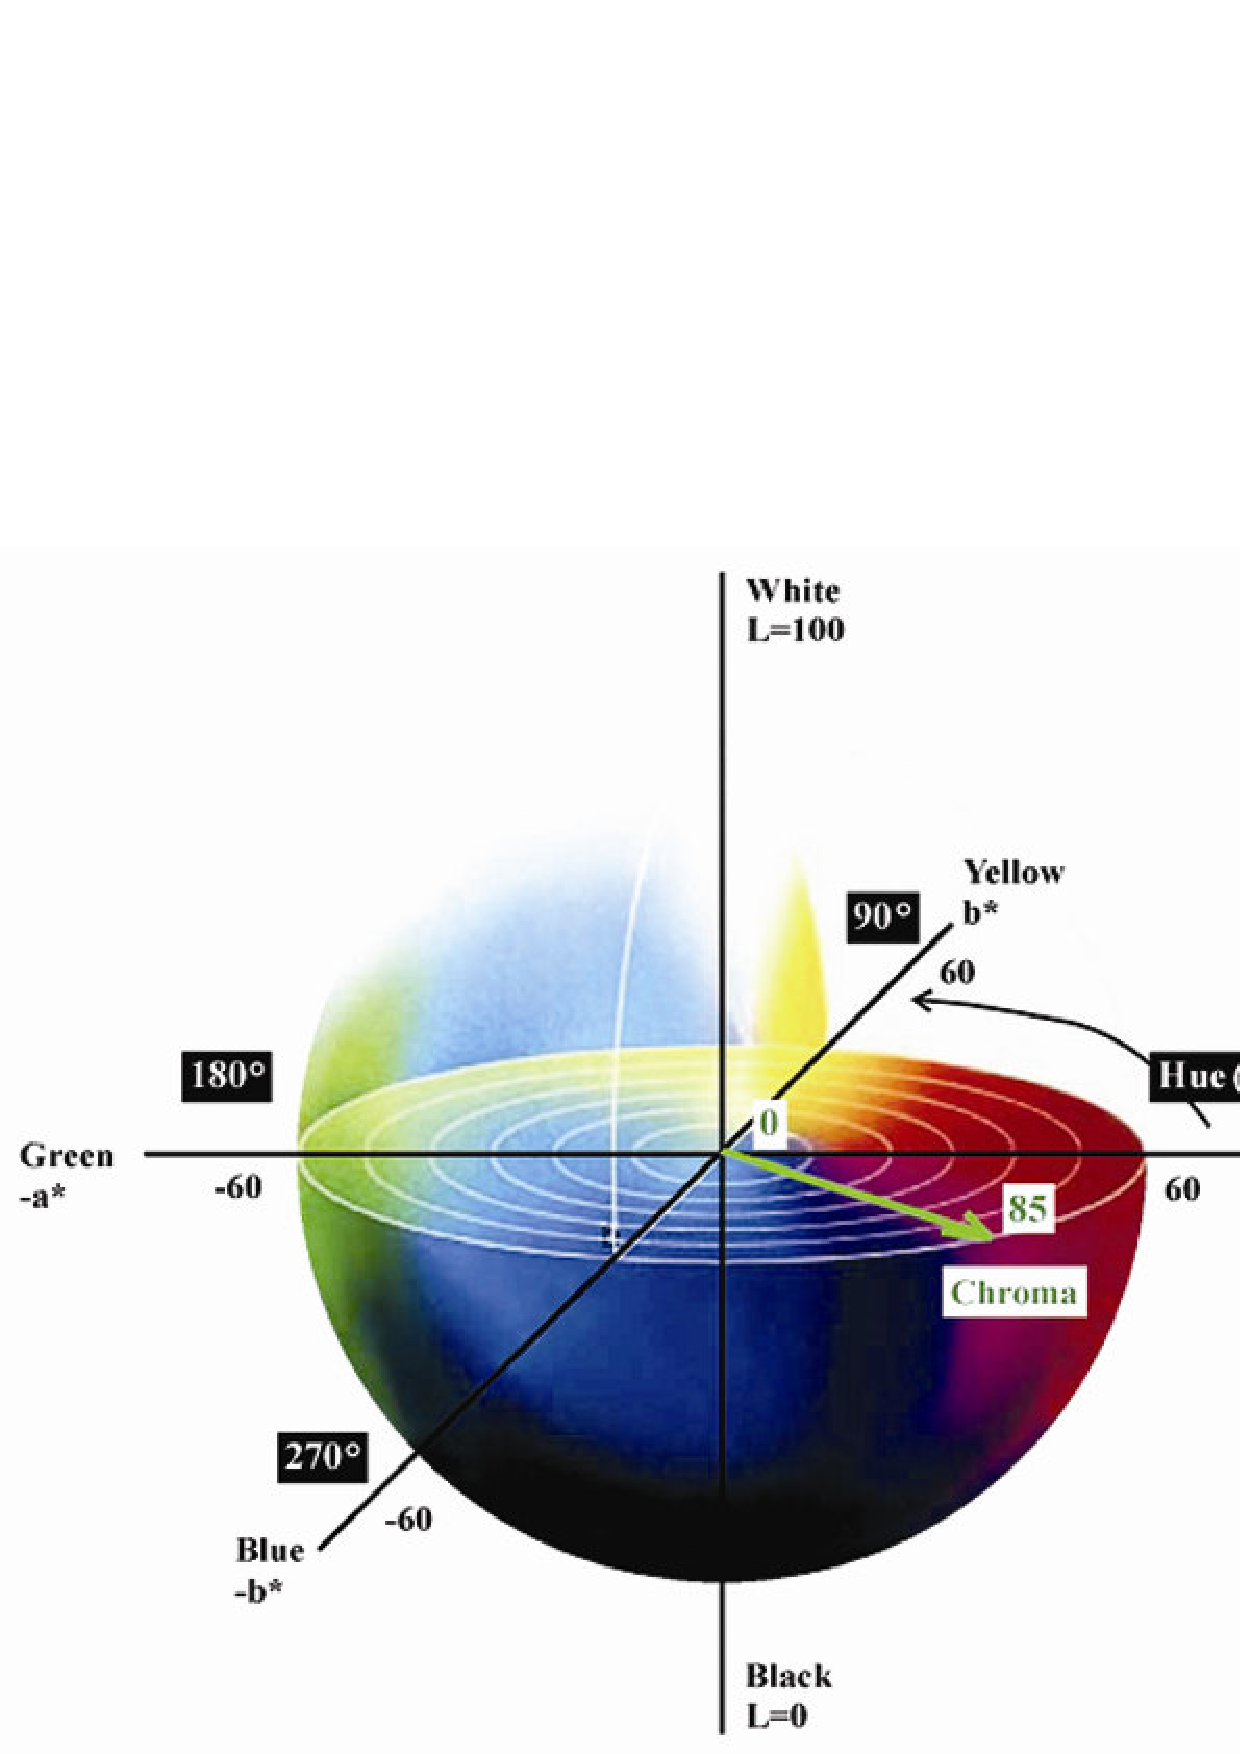
\includegraphics[width=.9\linewidth]{CIELab-colour-space.png}
		\caption{}
		\label{fig:Lab}
	\end{subfigure}%
	\caption{Colour spaces (a) HSV and (b) CIE-Lab.}
	\label{fig:colour-space}
\end{figure}

Two species of table grape were graded into five categories by Cavallo et al \cite{cavallo} after training a Random Forrest Classifier with features from the CIE-Lab colour space. The team calculated the mean and standard deviation of each channel and added the product of channels and ratio of channels to achieve a $92\%$ and $100\%$ cross-validation accuracies for Victoria and Italia strains, respectively.

A method to grade lemons based on colour and volume was implemented by Khojastehnazhand, Omid, and Tabatabaeefar \cite{khojastehnazhand} where the system could be calibrated to the specific requirements before assessment begins. By passing through fruit as examples to the system (and stored in a database), before using the example data as comparrison to the unseen fruit. The colour and volume information was calculated via HSI colourspace and simple geometry measurements where the volume estimation $R^2 = 0.9852$ and colour (ripeness) estimated accuracies of $95.45\%$, $100\%$, and $86.67\%$ for classes 1, 2, and 3, respectively.

For many leafy vegetables green is the predominant colour, therefore, extraction of the healthy components is made easy using the abovementioned colour spaces. In order to identify leafy vegetables Danti, Magdi, and Anami \cite{danti} utilised the RGB and HSI colour space channels by simply finding the mean and range (variance was eliminated as a non-determining factor) of each channel as features. The features were used to train a BPNN model which scored in the range of $92-100\%$ for all 10 leafy vegetables including dill, fenugreek, corriander, spinach and mint. 

RGB or a combination of RGB with other colour spaces also give significant results for certain applications. In order to grade palm oil fruit, May and Amaran \cite{may} simply analysed the RGB range of underripe, ripe and overripe fruit colour and determined accociated values correlating to the ripeness. Their fuzzy logic system achieved an overall accuracy of $86.67\%$ showing that this method is plausible for fruit ripeness determined by colour. A method to grade four different varieties of mango into four ripeness grades was implemented by Nandi, Tudu, and Koley \cite{nandi} by extracting colour features, and deriving other colour features at key points across length of the fruit. The features were then used with a simple Gausian Mixture Model (GMM) to achieve accuracies that rivaled expert humans. Blasco, Aleixos, and Molto \cite{blasco2} developed an algorithm that can detect 12 different types of common disease in citrus fruits. The method reduces the image to 32 colours before performing a region-growing method and could assess fruit from different batches, and even species, of citrus without adjustments. This was based on the assumption that unaffected fruit peel is relatively consistent, smooth, and blemish-free. An overall accuracy of $94\%$ was attained with some of the most devastating diseases scoring $100\%$ detection. 

Geometric calculations are a common approach to assessing shape, size, or volume as the scale and intestity are invariant which facillitates the background removal process, leaving a precise outline. This outline can then be precisely measured due to the fixed position of a calibrated camera. Properties such as minor and major axis can be used to calculate area (size) and lenth-to-width (elongation) of objects. Contour curvature, shape matrices, moments, and shape transforms such as Fourier and Wavelets can also be calculated from a well segmented image. 

Sandrina et al \cite{sandrina} implemented a method using geometric calculations to determine weight and shape of watermelons. Using logistic regression analysis they determined that good specimen shape could be well-described by an ellipsoid model with an $R^2$ of $0.97$. The weight of the watermelons was estimated by image analysis with an error of $2.42\%$. 

A review of assessment techniques for legume quality was conducted by Mahajan, Das, and Sardana \cite{mahajan} that found several species including lentils, soybeans, peas, chickpeas, beans, and honeylocust were assesed for their geometrical properties such as size and shape. Using a flatbed scanner for each of these projects, the methods consisted of simple thresholding and morphology to find the binary image before measuring. 



Fuzzy systems can offer generalisation and adaptability properties for grading based on feature simplification. A Fuzzy Inference System (FIS) takes raw data (crisp), transforms it into a simplified version (Fuzzification), and makes a prediction based on some knowledge, before transforming again (De-Fuzzification) back into a crisp value. Fuzzification methods may include bucketing, averaging, PCA, or windowing in order to reduce the dimensionality of data, usually giving the ability to assign simple rules to perfom the classification or detection.

Hasan and Monir \cite{hasan} developed a system to evaluate guava by use of a FIS. The fuzzy rules were based on functions of hue, saturation, and intensity of the images acquired of the fruit. Their method achieved an accuracy of $93.4\%$ which is an improvement over other classifiers such as naive bayes and multi-SVM. A method that used volumetric estimation in order to perform quality grading in fruit (apples, mango, orange, pomegranate, and strawberry) was designed by Jadhav, Singh, and Abhyankar \cite{jadhav}. Four cameras positioned at various angles and elevations were used to acquire the callibrated images of fruits before the volumetric calculations were peformed. This information is coupled with the colour values from the hue channel of HSV colour space to obtain a classification grade which is then passed to an FIS for final distribution into five grades from very poor to very good. All grades and all fruits achieved accuracies of $>98\%$. 

An adaptive neural-fuzzy inference system (ANFIS) developed by Zheng, Jiang, and Lu \cite{zheng} in order to detect bruising in Chinese bayberries as a function of Fractal Dimension (FD) and RGB values. The multiple input, single output Takagi–Sugeno fuzzy network consists of an input layer, fuzzification layer, rule layer, defuzzification layer, and output layer. The trained network could dicriminate between bruised and unbruised bayberries with an overall $90\%$ accuracy.



....




\subsection{Hand-selected Features}

The process of hand-selecting features is a common approach to help classifiers or networks to focus on the most important characteristics which determine class or defect. If the feature is a known conditional variable for the application then it can be a simple matter of extraction. For example, a particular fruit may have a distinctive disease indicator such as black spots or rough texture that can be exploited and visualised by applying image processing techniques. 

A tomato maturity level grading system developed by Wan et al \cite{wan} by projecting five concentric circles with different radii onto the fruit in order to extract the colour feature value. The correlated hue values were used to represent the maturity level before being trained on a 3-layer BPNN, achieving an average accuracy of $99.31\%$. Mebatsion, Paliwal, and Jayas \cite{mebatsion} found the best results when pairing morphological features with colour features in order to classify cereal grains into five common categories. They used a simple least-squared classifier obtaining a result of $98.5\%$ for barley, $99.97\%$ for CWRS (Canada Western Red Spring), $99.93\%$ for oat, and $100\%$ for rye and CWAD (Canada Western Amber Durum). Muhammad \cite{muhammad} also used hand-selected features when developing a method to classify date varieties. After an ellipse has been fit to the date image, features such as major and minor axis length, eccentricity, area, and texture descriptors were extracted and trained with an SVM classifier to achieve accuracies of $100\%$, $96.2\%$, $96.6\%$, and $99.6\%$ for the four varieties analysed. These results show that a small number of features, if properly selected, has the potential to perform extremely well under the right conditions.

Depending on the architechture used to classify the features, variance may be high especially when using neural networks. Features that best represent images for humans are not necessarily best represented for machine learning. Pereira et al \cite{pereira} hand crafted 21 colour features utilising three colour spaces (RGB, CIE-Lab, and HSV) in order to grade papayas into three maturity stages (MS). The mean values, pixel areas, and differential indexes between these colour spaces were obtained and classified by Random Forrest method resulting in an accuracy of $95.4\%$, $92.1\%$, and $84.4\%$ for MS1, MS2, and MS3, respectively. The team noted that it may be suitable for an industrial application in future. Szczypinski, Klepaczko, and Zapotoczny \cite{szczypinski} used an ANN classifer to attempt to discriminate between 11 different barley strains. 13 statistical metrics were obtained such as mean, skewness, second moment, and entropy in order to differentiate the varieties with an accuracy ranging $67\%$ to $86\%$. In an effort to grade persimmon fruit into three commercial maturity stages, Mohammadi, Kheiralipour, and Ghasemi-Varnamkhasti \cite{mohammadi} extracted features relating to RGB, CIE-Lab, HSV, and greyscale conversions before training both an LDA and QDA classifier to perform the categorization. The QDA model achieved an overall accuracy of $90.24\%$. Selected features chosen by Thendral and Suhasini \cite{thendral} improved the results, compared to no feature selection, for all tests performed whilst detecting defects in orange peel. They compared the performance of SVM, BPNN, and AANN finding that the AANN delivered the best testing results of $94.5\%$. Gill, Girdhar, and Singh \cite{gill} used a hybrid intelligent solution when developing a fruit grading method by means of a Genetic Algorithm merged with BP-ANN. The Back-Propagating (BP) method used to update weights in the network has a tendancy to become trapped in a local minima, leading to the idea of genetic algorithm (imitating natural evolution) coul overcome this problem. The results indicate that the hybrid system has increased accuracy ($93.33\%$) compared to a conventional BP-ANN ($73.33\%$).  



\subsection{Physical Property Analysis}

Hardware and physical properties may be exploited in some applications in order to avoid complex processing or improve results. Mutiple cameras, multiple spectrums and 3D imagery are examples of hardware employed in order to allow vision systems to capture details of the subject which may go unseen with conventional systems. 


Chui et al \cite{chiu} used a process of acquiring flourescence images - exiting the internal structure of the object in one wavelength, to emit light at a different wavelength - in order to detect mechanically-induced bruises on apples. They found that this method highlighted the bruised flesh, and extracted them by performing an image difference with a local adaptive binarisation method. 


Spectroscopy is a method of measuring the transmitted spectral signature of objects. By placing the light source on the opposite side, and not in direct view of the sensor, the transmittance can be measured to show unique properties regarding the internal structure of the subject. Figure \ref{fig:spectroscope} illustrates an example of a fruit spectrocopy system. 

\begin{figure}[h]
	\centering
	\includegraphics[width=0.7\linewidth]{spectroscope.png}
	\caption{Example of a spectroscope taking measurements from a fruit sample\cite{choi}.}
	\label{fig:spectroscope}
\end{figure}%


Matteoli et al \cite{matteoli} used a fibre-optic spectrometer to take measurements of peach fruits whilst performing destructive density testing in order to make predictions on new fruit non-destructively. They compared the output of a crisp versus fuzzy logic approach and found overall average accuracies of $60\%$ and $~80\%$, respectively, making the fuzzy system appropriate for the task. Choi et al \cite{choi} also used an NIR spectrometer to assess the internal qualities of pear fruit as well as CCD cameras to inspect the visible characteristics such as skin blemishes and colour. The spectroscope analysed the fruit for sweetness, acidity, hardness, and moisture before combining the two (visible and internal) features as classification variables for an ANN. 

A hyperspectral range of $400nm-1000nm$ was used by ElMasry et al \cite{elmasry2} to inspect various fruit by it's moisture content(MC), soluble solids(TSS), and acidity(pH). The resulting corellation coefficients of both the Partial Least Squares ($0.90, 0.80, 0.87$, respectively) and Multiple Linear Regression ($0.87, 0.80, 0.92$, respectively) proved the feasability of predicting these physical characteristics. They also measured three ripeness classes based on grey-level co-occurrence matrix (GLCM) analysis achieving $89.61\%$ classification accuracy.


Beyond the Near (NIR), Short (SWIR), lies the Mid (MWIR) Wavelength Infrared, and  Long Wavelength infrared (LWIR) which is the part of the spectrum ($3\mu m-15\mu m$)that objects near room temperature emit thermal radiation. This thermal information can be detected by specialised sensors and converted to correlated visible colours for humans to view as seen in Figure \ref{fig:thermal}.

\begin{figure}[h]
	\centering
	\includegraphics[width=0.5\linewidth]{thermal.png}
	\caption{A thermal image of two people showing the Long Wavelength Infrared (LWIR) range.}
	\label{fig:thermal}
\end{figure}%


Thermographic images in the wavelength range $3.4-5.2\mu m$ assisted Ginesu et al \cite{ginesu} to develop a thermal inspection system used to detect foreign bodies in produce items on a production line. Thermal imaging requires heaing or cooling in order to stimulate the subjects before being imaged sometime afterwards. Different materials heat transfer rates are varying, making the process of distinguishing, for example, sticks or stones from the edible items. They used a contrast enhancement and region-growing method to extract the highlighted regions from the greyscale thermal images.

On the opposite side of the visible spectrum resides ultraviolet, followed by X-ray wavelengths at which common medical and security inspections occur. X-rays are capable of penetrating objects in, for example, airport security allowing the users to visually inspect the contents of luggage. Medical applications include bone tissue and oegan imaging in order to help physicians make informed decisions about pateients. By choosing the optimal wavelength, many materials can be visualised internally including fruits and vegetables.    

Mathanker et al \cite{mathanker} analysed good and defective pecans using X-ray images. They compared AdaBooost and SVM classifiers finding that the AdaBoost average classification result of $92.2\%$ was the best performing.

....



\subsection{Hyperspecral/Multispectral Imaging}
\label{lab:lit_hyperspec}

As the spectral range of the eye is limited, camera sensors can be emeployed which can viualise wavelengths beyond these restrictions into the ultra-violet and infrared ranges. Figure\ref{fig:eye_sensor} shows the spectral response of the human eye versus CMOS and CCD sensors illustrating the extent to which the electronic sensor's range is greater.

\begin{figure}[h]
	\centering
	\begin{subfigure}{.9\textwidth}
		\centering
		\includegraphics[width=0.9\linewidth]{spectralresponse.jpg}
		\caption{}
		\label{fig:eye_sensor}
	\end{subfigure}

	\begin{subfigure}{.9\textwidth}
		\centering
		\includegraphics[width=.9\linewidth]{infra-red.jpg}
		\caption{}
		\label{fig:ifra-red}
	\end{subfigure}%
	\caption{(a) Spectral response of human eye (left) and CCD and CMOS sensors (right). (b) Infrared}
	\label{fig:spectrum}
\end{figure}%

Other sensors exist whose range is further into the infrared (SWIR, MWIR, LWIR, and FIR in Figure \ref{fig:ifra-red}), allowing many properties (usually internal) to be analysed.


Bruising in soft-skinned fruit and vegetables occurs if mishandled or exposed to excessive handling, reducing the quality for customers. Usually resulting from an impact, the moisture comes to the surface and therefore can be differentiated from the sourround soun tissue by means of analysing several water absorbtion bands in the visible and NIR regions. Hyperspectral imaging and PCA reduction used by Che et al \cite{che} provided an accurate method to extract bruise regions from apple images. Using two characteristic wavebands at $675nm$ and $960 nm$, they analysed the fruit $0h$, $12h$, and $18h$ after bruising impact and found that the Random Forrest classifer performed best at $99.9\%$ average accuracy. Qiang and Mingjie \cite{qiang} used hyperspectral imaging  in the range of $408nm-1117nm$ in order to detect bruising in kiwi fruit. They were able to detect the bruising through the thick peel where human vision could not with an overall error rate of $14.5\%$. 

Munera et al \cite{munera} developed a system using visible and NIR hyperspectral imaging in order to grade persimmon fruit by firmness, maturity level, and astringency. Using CIE-Lab colour space, they found that the $L$ and $b$ coordinates decreased whilst the $a$ coordinate increased with maturity, allowing good corellation with colour parameters such as $H(R^2 = 0.83)$, $G(R^2 = 0.82)$ and $h(R^2 = 0.81)$. Ratios of the colour channels were also analysed with results achieving $a/b(R^2 = 0.83)$, $G/R(R^2 = 0.83)$, and $a/L(R^2 = 0.83)$. Three wavelengths were chosen as optimal ($580nm$, $680nm$, and $1050nm$) in order to perform the ripeness tests with all accuracy $>94\%$ using LDA, QDA, and SVM classifiers. The astringency test used the same classifiers and resulted in $>90\%$ for all, and $>95\%$ for the QDA method. This indicates the ability of non-destructive assessment of the maturity, firmness, and astringency of these fruits is valid.

In order to grade cherries into three maturity stages, Li et al \cite{li} analysed characteristics in terms of Soluable Solids Content (SSC) and acidity (pH) with hyperspectral imaging in the range of $874nm-1734nm$. Two full-band methods were tested, namely, principal components regression model and partial least squares regression model both with similar accuracy. A genetic algorithm (GA) was used to reduce complexity in bandwidth by reducing the full spectrum to 54 optimal bands for the SSC model and 28 for pH, and reported a $96.4\%$ total accuracy.  

Using hyperspectral imaging ranging from $950nm$ to $1650nm$, Lee et al \cite{lee} exploited the ability of NIR wavelengths to detect bruising in pears. By investigation it was found that the waveband ratio of $1074nm/1016nm$ higlighted invisible bruises which could then be extracted using thresholding with a $92\%$ accuracy. 

....







\subsection{Strawberry Image Processing}

Strawberries are a delicate fruit with an unprotected, soft, edible flesh, and very susceptible to damage if mistreated, handled too much, or even transported carelessly. The outer flesh of the berry is pinned with seeds creating higher surface friction, coupled with the incredibly soft exterior, creates challenges in terms of handling during picking, packing, and distribution. This is conversely true for fruits such as mango, watermelon, oranges, kiwi, and banana, for example, which have a protective, smooth layer of peel to protect the flesh inside, seen only by the consumer. Some success has been made in machine vision for strawberries, with examples in robotic picking, picking and grading, and grading on a production line. 

Brosnan and Sun \cite{brosnan} performed a review of agricultural vision systems including apple grading, orange stem detection and sweetness correlation, unsplit pistachio nuts, tomato size, colour, and shape properties as well as seedling health, peach and pear maturity levels, and automatic fruit harvesting. The team also reviewed vegetable inspection methods such as musshrooms and potatos, as well as wheat, rice and corn. The team noted 2 methods for analysing strawberry shape and size, taking one of the teams $1.18 s/berry$ and noting that fruit quality is dependant on a number of pre-harvest and post-harvest processes. 

Using a conveyor system, L. Xu et al \cite{xu} achieved very good results in classifying shape, ripeness, and size. The measurements are attained by using a K-means clustering method to find 7 vertical and 7 horizontal axis lines. Size feature was calculated by performing experiments to find the ratio of pixels/mm and simply dividing the pixel measurements of the berry by this ratio. Using the CIELAB colour space, a dominant colour was found in the berry by means of a histogram windowing method. Similarly, Liming and Yanchao \cite{liming} developed a strawberry grading method and mechanical system that requires manual loading of single strawberries on a converyor belt before using colour features and k-means clustering to grade the fruit into shape and colour classes at a rate of approximately $2.5s/berry$. 

S. Yamamoto et al \cite{yamamoto2} used simple RGB techniques to define the ripeness of strawberries when developing an automated harvesting machine. They used a combination of green, red, and white LED's in order to illuminate the strawberries in specific wavelengths, giving better judgement on whether to pick or not based on ripeness. The harvesting machine was designed to be stationary with the fruit being presented to the machine via moving beds, which implies a large amount of fabrication and process chgange would be required to persue this method. The authors reported high harvesting rates ($67.1\%$) compared to that of other more conventional harvesters, however, their system was succeptible to fruit damage and requires improvement in harvesting speed. Hayashi et al \cite{hayashi} reported a rate of $11.5s/berry$ using their automated harvesting machine. The end-effector designed by the team used a peduncle cutter in conjunction with a suction cup to pick the fruit from the plant and place it in a padded tray as shown in Figure \ref{fig:strawberry_picker}. The HSI colour space was used to generate a maturity level when grading the fruit to be picked. By creating acceptable and unacceptable sections of the average hue, saturation, and intensity channels, they could discern $>80\%$ ripeness with an accuracy of $41.3\%$.

\begin{figure}[h]
	\centering
	\includegraphics[width=0.9\linewidth]{strawberry_picker.png}
	\caption{Strawberry picking machine from \cite{hayashi} (a) demonstrating end-effector mechanism (b) placing strawberry into the foam tray.}
	\label{fig:strawberry_picker}
\end{figure}%


Strawberry cultivar are numerous around the world and their distinguishing features seem only obvious to expert humans as shown in K. Yamamoto et al \cite{yamamoto} when they implemented a method to distinguish between 21 different strawberry cultivars. They found that when using a single feature such as colour, shape, or size, the average accuracy was very poor at $<42\%$. However, when these three features were used in conjunction, the discriminant analysis classifier performed better at $68\%$. This shows that strawberry cultivars are not simply classified due to the inter-species colour and form having similar features. 


EMasry et al \cite{elmasry2} used multi-spectral imaging in order to determine the moisture, soluable solids, and pH levels in order to grade the ripeness of single strawberries. They found broadband absorbtion bands, in the case of underripe fruit, at 500, 680, 840, and $960nm$. The bands at 840 and $960nm$ were found to represent sugar and water absorbtion which was used to determine factors that would usually require destructive testing. The same results were found by Tallada, Nagata, and Kobayashi \cite{tallada} using an NIR hyperspectral system, they analysed and asessed the firmness of strawberries by non-destructive imaging. By taking acquiring images from $640nm-1000nm$ in steps of $5nm$ they were able to dertermine the optimal wavelengths to estimate firmness accross three grades of ripeness. The results had a correlation of $0.786$ and standard error of $0.350MPa$ using $685nm$, $865nm$, and $985nm$. They calculated formulas to generate heat maps of the firmness distribution (pseudo-colour), as shown on the ripe and underripe examples in Figure \ref{fig:multispec_strawberry}. This result is expected given the deep red colour of the top specimen versus the half white, and red example.

\begin{figure}[h]
	\centering
	\includegraphics[width=0.5\linewidth]{multispec_strawberry.png}
	\caption{Pseudo-coloured strawberry heatmap showing the white area of the berry being firmest and the red area softest.}
	\label{fig:multispec_strawberry}
\end{figure}%

Zhang et al \cite{zhang} used a hyprspectral imaging system in two ranges - $441nm-1013nm$ and $941nm-1578nm$ to assess the ripeness of strawberries into three categories. Using PCA for reflectance processing and texture components at optimal wavelengths to form the feature set, they trained an SVM classifier achieving overall classification accuracy of $85\%$. 

 




\subsection{Real-time Systems}

One of the most challenging aspects of developing vision systems designed for quality inspection is the process of production implementation. Accuracy, speed, safety, power, robust design, operator use, control mechanisms, and signals must all be considered in order to progress from bench design to production-ready. Control mechanisms and speed of processing are the most prominent of these considerations, with many solutions using simplified processes.

Fruit and vegetables are generally graded by the ripeness or rediness to eat, based in predominance on their colour, size, and texture. Therefore many solutions to real-time grading use simple colour algorithms, many in combination with size and texture estimation. Sofu et al \cite{sofu} designed and automatic apple sorting system which processed at a rate of $54,000 apples/h$ acheiving an accuracy of $79\%$. A simple descision tree was used to classify the specimens according to colour, size, stain and weight before sorting the apples using opening bowl mechanisms. Their system, described in in Figure \ref{fig:apple_system}, shows the lighting box enclosure, operator control panel and PLC display, and control system of opening bowls in the foreground of the diagram.

\begin{figure}[h]
	\centering
	\includegraphics[width=0.7\linewidth]{apple_system.png}
	\caption{Apple sorting system \cite{sofu} showing the lighting box with cameras in the background with opening bowls in the foreground.}
	\label{fig:apple_system}
\end{figure}%

A fig sorting system developed by Baigvand et al \cite{baigvand} could successfully categorise the figs into five grades with accuracies up to $95.2\%$, processing at a rate of $90kg/h$ and sorting each into separate bins using air nozzles. The team created indices related to colour, size, and the area of the split, seen on each fruit, applying a rule-based method to determine the graded category. 

In order to remove the green calyx from strawberries, Lin et al \cite{lin} used a waterjet cutting system guided by machine vision. The strawberries were fed into the system using roller rods to align and separate before using CIE-Lab colour space to segment the berries from the calyx. A series of geometric calculations guide the cutting system with the optimal cut line. Their machine was designed to process berries bound for ice cream, yoghurt, jucing, and jam markets instead of being packaged for sale as fruit, meaning that condition, bruising and ripeness was not of concern as much as removing the green leaves.

Hyperspectral and mutispectral implementations can help systems to assess products in real time due to their abitlity to see what the human eye, or regular cameras can detect. This advantage can provide information which simplifies the processing of images, for example, the use of NIR wavelengths can uncover invisible defects (as discussed in Section \ref{lab:lit_hyperspec}). Lee et al \cite{lee} implemented an industrial date grading machine capable of processing $72,000 dates/h$ with an $87\%$ accuracy measured. They acquired images in NIR wavelengths ranging $750-1200nm$ by use of an NIR-extended CCD camera and a high pass filter to block wavelengths lower than $750nm$. Processing at a rate of $20 fruit/s$ ,these wavelegths provided good background segmentation, added to the amplification of delaminated skin features which determine quality. The amount of delaminated skin was calculated, after morphological operations, and compared to the size of the entire fruit to give a percentage and a grade from 'A' to 'E'. 

When implementing systems in production environments, the rate of production (and limited space constraints) sometimes require inventive solutions to be implemented in order to acheive the desired outcomes. Aleixos et al \cite{aleixos} developed a commercial citrus grading system which used a combination of transmissive and reflective lenses in order to image the same scene with two cameras. One RGB and one NIR camera were used to acquire images of citrus fruits at a rate of $5 fruits/s$ before assessing each for size and colour and surface defects. The size estimation had $<2mm$ error with colour grading for oranges, lemons, and manderins reaching $94\%$, $93\%$, and $94\%$, respectively.

Machine vision can outperform humans depending on the task involved. Particularly for borderline cases a machine has finite thresholds inplace to ensure consistent outcomes. Estimating ripeness colour, areas of scattered blemishes, and measurements can be difficult and/or subjective between human experts but easily calculated with vision systems. A meat marbling grading system developed by Barbon et al \cite{barbon} trained a k-NN classifier to grade meat samples in $<1s$, which is an improvement on human gradation time of $11s$. Their method was suitable for a range of lighting conditions and animal type due to the illumination normalisation and contrast enhancement processes before classification attaining results of $81.59\%$ and $76.14\%$ for bovine and swine, respectively. 


No strawberry grading real-time systems...



\subsection{Machine Learning / Deep Learning Methods}


Machine learning is a branch of computer science and AI that uses an iterative 'learning' approach to building a classifier model. The model's weights are updated by an algorithm that, given any training set ($x_1, y_1$), ($x_2, y_2$), ... , ($x_n, y_n$), can learn a function $y = f(x)$ to make prediction of an unseen $x_{test}$ variable. Deep Learning refers to the depth of the network or number of layers the model has. Using a deeper network allows for multiple convolutions in a CNN and therefore better abstraction, albeit more computationally expensive. A range of methods have been investigated from very basic MLP networks, SVM, and ANN to more complex architectures such as CNNs.


Comparison of MLP neural network and Discriminant Analysis (DA) performed when grading golden delicious starfruit by Abdullah et al \cite{abdullah} found that the colour attributes were more accurately classified by DA, with resulting $95.3\%$ and $90.5\%$ for DA and MLP, respectively. The method used to extract colour features based on hue values $10-74$ were improved with the DA classifier using Wilks-lambda reduction, however the MLP result was unchanged. In order to classify shape characteristics, Fourier discriptors were used generating a $100\%$ accuracy.


Zhang et al \cite{zhang} used an FNN to classify a fruit dataset created via on-site collection and on line. After background removal, the 79 features that had been constructed based on colour, texture, and shape were obtained before being reduced via PCA to 14, and used to train the network using 5-fold cross validation. The classification accuracy of $89.1\%$ outperformed other methods tested such as BP, momentum BP, and GA. 

Even for simple networks, the relationship of problem domain to network architechture is not well defined in terms of accuracy. Zuniga et al \cite{zuniga} used a supervised learing approach with small ANNs in order to grade grape seeds from images acquired scattered over a flat-bed scanner. Using a process of analysis and trial and error, the optimal number of neurons is found and a classifier trained giving total accuracy of $86\%$ for the test set. An apple grading system developed by Vakilian and Massah \cite{vakilian} used a 3-layer ANN whilst grading Golden Delicious and Red Delicious varieties with respective overall accuracies of $89\%$ and $92\%$. Extracting the images textural (mean and variance of energy values) features before training separate networks for each apple variant. Finally, they invstigated the width of the ANN's middle layer ranging the architechture of the network from $2-2-4$ to $2-20-4$ finding the optimum width of $2-12-4$. 

Conversely, Wang et al \cite{wang} had perfect results using a similar architecture whilst developing a method to find worm-eaten holes in chestnuts. Using Sobel edge detection and using the resulting, filtered region to train a BP network. Conversion occured after only three iterations and achieved $100\%$ for both good and wormhole classes.

When using hyperspectral/multi-spectral data, it is possible to extract internal attributes such as structure, soluable solids (sugar content) and pH levels depending on the subject and wavelength range. Sugiyama et al \cite{sugiyama} were able to detect stems and leaves (foriegn objects) from hyperspectral blueberry images. They found that the foliage was easily extracted at particular wavelengths (1268 and $1317nm$) and were then able to perform a discriminant analysis between the two wavelengths in order to segment and highlight the defects.

Extreme Learning Machines (ELM) have gained popularity in the last few years. An ELM is used to train a single hiden layer feed neural network (SLFN) in a more efficient way by performing a random feature mapping and a least squared formula based linear regression \cite{peng}. Luo et al \cite{luo} used a kernel extreme learning machine to create a mulit-label classifier used in applications where designators are applied to an unseen object. Xu et al \cite{xu} used an ELM to continuously modify it's classifier in a dynamic process due to concept drift in applications. Extra nodes are added when an alert flag is set in the algorithm, and if the error rate drifts too far, the classifier is erased and a new classifier is trained. A novel twin ELM algorithm was used by Wan et al \cite{wan} to train two classifiers simultaneously by creating two non-parallel hyperplanes. 

ELM have proven to be an efficient and accurate method to train classifiers due to the least square formulation approach to find the solution, opposed to the first and second order gradient descent method \cite{yavs}. the ELM out-performs other classifiers such as SVM and k-NN which have been tested independently \cite{yavs, wan, peng}, due it's combination of fast training times, testing times, high accuracy, and low error rate. Several applications were able to implement ELM in real time systems due to these factors \cite{xu, yavs}.  

Mohammed et al \cite{mohammed} used a novel Bi-directional two Dimensional Principal Component Analysis (B2DPCA) in conjunction with an Extreme Learning Machine (ELM) in order to greatly improve facial recognition accuracy in popular face datasets. The B2DPCA technique proposed keeps the data in matrix form as opposed to vector form for PCA processing, and the ELM is a variation of a feed forward, single hidden layer neural network, with the main difference being assignment of random input weighs and hidden layer biases which transforms training the network into a linear system. Zheng, Fu, and Ying \cite{zheng} used an Extreme Learning Machine (ELM) to classify spectroscopic data acquired from four different foods - coffee, meat, oil ,and fruit. The results indicate good results for the coffee, meat, and oil with $100\%$, $97.78\%$, and $97.35\%$ accuracy, respectively, whilst the fruit classification was less accurate achieving $95.05\%$. They compared all the datasets and ELM by applying five different methods including KNN, DA, and ANN, finding that SVM was the most appropriate. 


\subsubsection{Support Vector Machines}


SVM can be considered a type of neural network that has only one hidden layer of neurons. The SVM attempts to create a hyperplane between the feature sets of each class. The support vectors are formed as non-zero coefficients of the data points found after processing the training set. If the margin is large between the hyperplane and each class, the system is said to be a stronger SVM classifier and should produce good results as explained by Osuna, Freund, and Girosi \cite{osuna}. Standard SVM inherently is incompatible with large datasets which suits applications with a small set of training examples. This is due to the $O(m^3)$ training time and $O(m^2)$ space complexity where $m$ is the size of the dataset \cite{tsang}.

Given a set of training data {$(x_i, y_i), x_i \in X^n, y_i \in (-1,1), i = 1,2,3,...,n$} th SVM kernel attempts to solve the hyperplane decision boundary equation:
\begin{equation}
w \cdot x + b = 0
\end{equation} 
giving
\begin{equation}
w \cdot x + b \geq 0, \quad \textrm{for} \quad y_i = +1
\end{equation}
and
\begin{equation}
w \cdot x + b < 0, \quad \textrm{for} \quad y_i = -1
\end{equation}

Here, $w$ constitutes the variable vector and $b$ the bias vector. Beginning with the kernel function $K(x, x^\prime)$ which obtains the non-linear mapping $\Phi(x)$, the solution takes the form:
\begin{equation}
f(x) = b + \sum_{i=1}^{m} y_i \alpha_i K(x, x^\prime)
\end{equation}
which is the summation of each support vector of length $m$, the respective $y$ values, Lagrangian multiplier ($\alpha_i$), and the kernel $K(x, x^\prime)$. Figure \ref{fig:SVM} shows an example of a hyprplane desicion boundary set by finding the solution above.

\begin{figure}[h]
	\centering
	\includegraphics[width=0.5\linewidth]{SVM.png}
	\caption{A 2D example of SVM yperplane separating two classes. The examples on the boundary are considered the support vectors.}
	\label{fig:SVM}
\end{figure}%

SVM kernels are generally set to be one of the following:

\begin{itemize}
	\item Linear - $K(x, x^\prime) = x_i \cdot x_i^\prime$
	\item Polynomial - $K(x, x^\prime) = (\gamma x \cdot x^\prime + r) ^d, \quad \gamma > 0 \quad$
	\item Radial basis function (RBF) - $K(x, x^\prime) = e^{-\gamma\|x-x^\prime\|^2},  \quad \gamma > 0 \quad$
	\item Sigmoid - $K(x, x^\prime) = tanh((\gamma x \cdot x^\prime + r)$
\end{itemize}

with $\gamma = \frac{1}{2\sigma^2}$, and $r$, and $d$ are kernel parameters. 


An SVM classifer trained by Sabri et al \cite{sabri} was able to classify ripe and unripe palm oil fruits with an accuracy of $96.59\%$. They compared three methods of feature extraction (Colour histogram, colour moment, and colour correllogram) and two classification methods (SVM and Naive Bayes) in order to find the best results with SVM prevailing. Chen et al \cite{chen} performed an SVM parameter search to find the best combination whilst colour grading beef fat. They segmented the fat by use of boundary tracking, thresholding, and morphology achieving $97.4\%$ classification accuracy. Mizushima and Lu \cite{mizushima} used SVM to generate greyscale images that increased the contrast of Golden Delicious apples for segmentation purposes, before again using SVM to classify them into three grades reporting $1.42\%$ error accross all three classes. They also achieved fast processing speeds of $1.5ms$ using a $3.4 GHz$ CPU showing that SVM is capable of very fast and accurate predictions. 

However, SVM was not the predominant classifier when Alfatini et al \cite{alfatni} designed a palm oil grading application. The method consisted of using a basic grey level aura matrix (BGLAM) technique to extract features followed by an ANN classifier. After assessing ANN, KNN, and SVM classifiers, the best results were realised using the ANN with accuracy of $93\%$ and speed of $0.4s$. An ANN was also used by Bhatt and Pant \cite{bhatt} when grading apples based on size, colour, and external defects. Seven selected features were used (3 colour features, 1 size, 1 damage, 1 symmetry, and 1 weight) to train the ANN achieving $90\%$ testing accuracy. 


 


\subsubsection{Deep Learning}

Machine learning is a broad term that encapsulates Artificial Intelligence (AI) techniques adopted from many approaches, and can be defined as any  computer program that can perform tasks, after having been trained,  without having to be explicitly told to \cite{langley,shavlik,mohri}. In other words, the program can adapt and configure itself to specific conditions in order to make decisions, improve accuracy or efficiency, control systems, and predict outcomes among many other uses. The \textit{learning} is a term that refers to the process of training a program to perform a task. Given a training set $(x_i, y_i)$, $x\in X$, $y\in Y$ of inputs and outputs, the program must derive a function $f$ that satisfies $f(x_i) = y_i$ for all $i$. A very large training set will improve accuracy, however, this may result in extremely long periods of training (weeks in some cases \cite{bottou}), or over-fitting problems. Training can be sped up, however, by increasing computational power such as high-end GPU's or supercomputer systems.

Neural Networks, in AI, are a commonly implemented method for perfoming many operations and are made up of one or more layers of neurons as shown in Figure \ref{fig:neural_net}. The layers in this image are fully connected, meaning that each neuron in the layer $L_n$ takes inputs from the layer at $L_{n-1}$, and can output to the layer at $L_{n+1}$, however, neurons in the same layer may not be connected. This is the most common approach, although, sometimes it is beneficial to avoid fully connected layers. An SVM classifier can be thought to be modelled as a single layer NN, and other terms have evolved such as Artificial Neural Networks (ANN) and Multi-layer Perceptron (MLP). However, more complex topologies can be constructed with the addition of convolutional steps between layers, known as a Convolutional Neural Network (CNN) and the term Deep Learning or Deep Neural Networks (DNN) where the depth is seen in the number of connected layers.  

\begin{figure}[h]
	\centering
	\includegraphics[width=0.8\textwidth]{neural_net.jpeg}
	\caption{Neural network topology with 2 hidden layers \cite{smith}.}
	\label{fig:neural_net}
\end{figure}

Figure \ref{fig:neural_net} shows the flow of information through the layers in a neural network. Each of the inputs $Xn$ is fed to the first hidden layer with a relevant weights $W_{i,j,k}$ and biases $B_{i,j,k}$ associated for each of the neurons. Each neuron sums the weighted inputs and the value interpreted by the activation function is sent to the next layer, with yet another set of weights and biases, for each neuron. Activation functions are usually in the form of linear $y=x$, sigmoid $y=\frac{1}{1+e^{-x}}$, or hyperbolic tangent $y=\frac{1-e^{-2x}}{1+e^{-2x}}$.


For an activation function $f$, the $i$th neuron $a$ is given by:
\begin{equation}
a_i = f\bigg((w_i^0 x_i^0 + b_i) + (w_i^1 x_i^1 + b_i) + (w_i^2 x_i^2 + b_i) + ... + (w_i^n x_i^n + b_i)\bigg)
\end{equation}

or by summation: 
\begin{equation}
a_i = f\bigg\{b + \sum_{i=0}^{n} w_i x_i \bigg\}	
\end{equation}

After computing these neuron activations, the Back-Propagation (BP) process is used in order to update the weights and biases. This is done by firstly assessing the cost of the output of the network versus the training sample value ($y_i$). The cost $C_{w,b}$, where $w$ is all weights within the network, and $b$ all biases, is given by:
\begin{equation}
C_{w,b} = \frac{1}{2n} \sum_{i=0}^{n} \|y_i - a\|^2	
\end{equation}
This cost function is minimised (training process) by using methods such as gradient decent to arrive at the optimal solution, where the small change in cost $C$ takes the form:
\begin{equation}
\Delta C \approx \frac{\partial C}{\partial w} \Delta w + \frac{\partial C}{\partial b} \Delta b	
\end{equation}

These parameters are calculated and updated at each pass (epoch) and therefore may be set to some value initially, but may only be changed by the computations thereafter.

Machine learning programs have been adapted in areas such as text categorization \cite{sebastiani}, handwriting recognition \cite{bottou,bahlmann}, facial recognition \cite{bartlett,bartlett2,mohammed}, medical diagnosis \cite{shipp,ye,dreiseitl}, gesture recognition \cite{lustrek,rautaray}, image classification and computer vision \cite{chapelle,ciresan,krizhevsky}, search engines and chat bots \cite{boyan,graepel,jia}, marketing/data mining \cite{cui,bose}, and an endless amount of other applications. This technology has seen rapid popularity and growth due to the flexibility and adaptiveness of such algorithms, which allows it to be used by many companies and individuals to improve systems performance. 

In recent years, self-driving cars, trucks, taxis, mining equipment, and UAVs are using ML to process images, and interpret sensor data, to recognise elements and obstacles required to operate safely. This autonomous revolution is driving machine learning research and development in great popularity \cite{lecun}. Starting with DARPA, large companies such as Google, IBM, and Microsoft have invited hobbyists, programmers, and computer scientists - anyone who has the ability - to contribute to their AI systems, processes, and libraries with solutions to problem domains they set \cite{tensorflow,cortana,udacity,xprize}.


A comparison of six deep learning architectures performed by Koirala et al \cite{koirala} in order to grade mangoes showed that all networks can perform with accuracy $>90\%$. The architectures evaluated were Faster R-CNN(VGG) (original version, and input dimension altered), R-CNN(ZF) (original version, and input dimension altered), SSD (original version, and input dimension altered), YOLOv3 (altered), YOLOv2 (original version, and input dimension altered), YOLOv2(tiny) (original version, and input dimension altered), and a specialised network based on YOLO MangoYOLO. The MangoYOLO network has slightly higher F1 score of $96.8\%$ with the inference speed at $<70ms$ for all networks using an NVIDIA GTX 1070 Ti GPU and $32GB$ of RAM.

Ma et al \cite{ma} developed a CNN to perform disease recognition among cucumber leaves including anthracnose, downy mildew, powdery mildew, and target leaf spots. The disease is more easily and less laboriously found on the leaves of the cucumber plant as opposed to the fruit itself. The team used a DCNN to perform the detection with results of $93.4\%$ which outperformed alternative algorithms such as SVM, Random Forrest, and AlexNet.

   


....






\subsection{Control Systems}

Vision systems have been utilised on many production lines since the early 1980's \cite{kruger}. Computers represent a medium to perform a consistent, verifiable approach to monitoring, recording, and quality control of produced items. These items may be susceptable to damage, contamination, manufacturing errors, poor quality, out-of-specification features, or defects and require separation from good quality produce. Depending on the goods being monitored, there may be an option to rework, correct, repack, or remake the defected instances, therefore, the control systems will differ greatly between production lines.   

The fruit grading system by Kondo \cite{kondo} used two robot arms with 3 DOF performing a series of tasks to determine colour, size, shape, and defect. The robots alternate using suction cups to pick up 12 fruit at once in order to acquire images from the above, below, and 4 sides before pushing them into the corresponding lines. 12 camera systems in total are used, with others guiding the manipulators. This, and the project by Michalosa et al \cite{michalosa} combining mobile robots with tooled manipulators serves as examples of precision, complex, robotic control systems. However, as agricultural production line items generally are not required to be assebled or involve precise movements, control systems are relatively easy to implement, without the need for complexities such as several degrees of freedom or specialised tooling to perform the task of quality control.  

Blasco et al \cite{blasco} performed grading of pomegranite arils into five categories - White, Pink, Red, Brown , and Unwanted using several pnuematic air nozzles to eject the arils into their appropriate outlets. The system can grade a maximum of $75kg/h$ using six narrow conveyors and is highly dependant of the feeding unit to uniformly distribute the arils on the conveyor belts. As the air nozzles have a conical burst of air, incorrect rejections can occur if they are too closely distributed, or if external factors cuase the arils to roll between the vision system and control. Pneumatic air ejectors helped Nouri-Ahmadabadi et al \cite{nouri-ahmadabadi} in order to grade pistachio kernels from unwanted shells. The system also required a good separation of individual items on the conveyor in order to correctly eject the affected instances. The sorter requyired an $8mm$ separation and could process $22.74kg/h$ with an accuracy of $94.33\%$. 

A date grading system by Al Ohali \cite{ohali} used electro-mechanical sorting strips placed at the end of the conveyors which guide the fruit into different grades. This type of control must have even larger spacing due to the mechanical movement followed by a return. Systems developed such as Sa'ad et al \cite{saad} mango shape and weight grading project used push/pull actuators to remove defect items and is akin to conveyor process control (i.e. conveyor separation, interleaving conveyors, conveyor gates, etc). Makky and Soni \cite{makky} developed a grading machine for oil palm fresh fruit bunches using stepwise discrimination in order to classify into accept and reject classes with an average success rate of $93.53\%$. Their design (and in-field implementation) employed a gate driven by a limit switch to separate the good fruit from the rejected.




\subsection{Summary}





%%%%%%%%%%%%%%%%%%%%%%%%%%%%%%%%%%%%%%%%%%%%%%%%%%%%%%%%%%%%%%%%%%%%%%%%%%%%%%
%%%%%%%%%%%%%%%%%%%%%%%%%%%%%%%%%%%%%%%%%%%%%%%%%%%%%%%%%%%%%%%%%%%%%%%%%%%%%%
\newpage

\section{I - Design and Prototype}

\subsection{Design}

\begin{figure}[h]
	\centering
	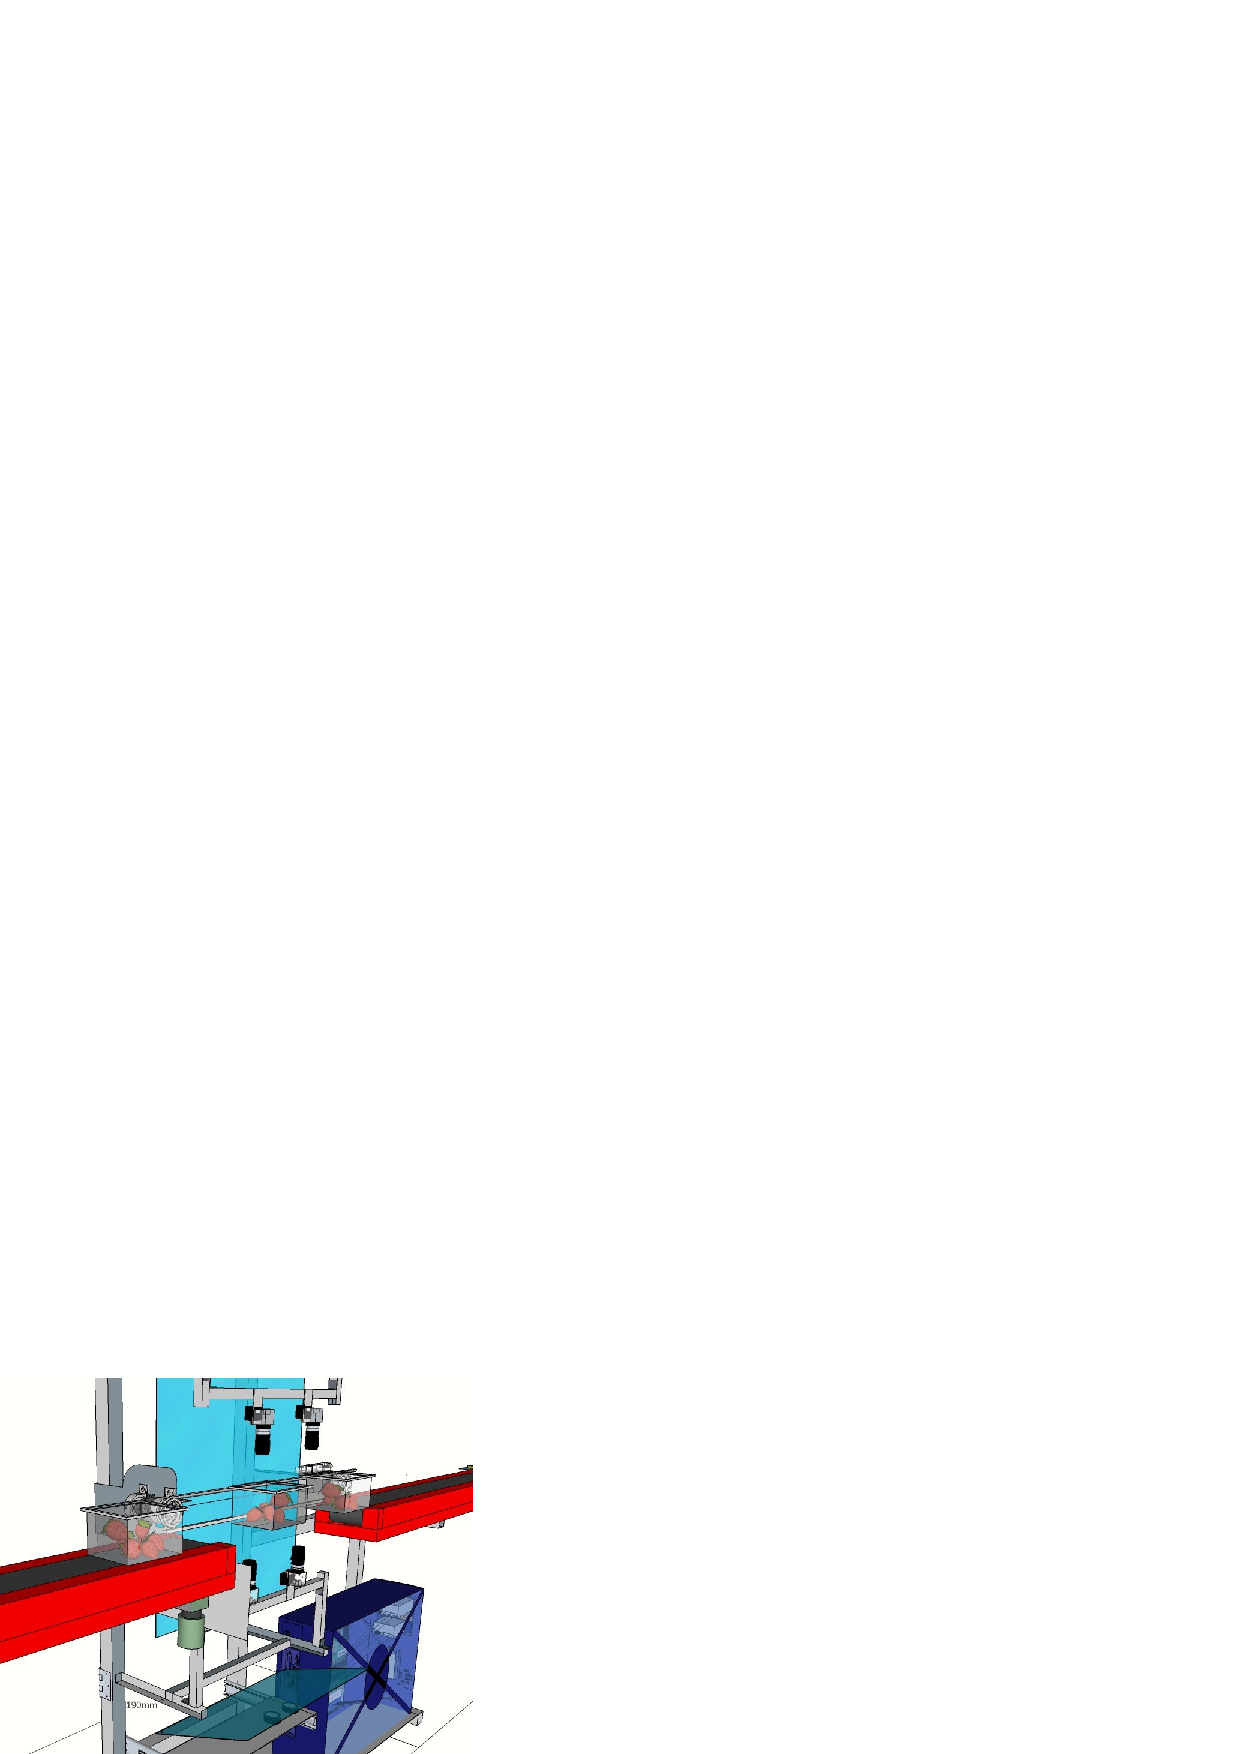
\includegraphics[width=.8\linewidth]{QAS_cross_sec.jpg}
	\caption{}
	\label{fig:cross_sec}
\end{figure}%



\subsection{Project Challenges}

\subsubsection{Punnet Imaging}

Shiv Ram Dubey and Anand Singh Jalal \cite{shiv} investigated fruits and vegetables as well as some fruit diseases using a multi-class SVM classfiers as a solution. Qiang LÜ and Mingjie TANG \cite{lu} devised a method for identifying Kiwi fruit, which had hidden bruises under the skin, by using hyper-spectral imaging and a parallelepiped classification approach. These experiments, as well as other work \cite{elmasry2,chiu}, have used a static imaging system. That is, the subject was stationary and usually had a clean, flat, un-obscured background that makes the process of segmentation quite trivial. ElMasry et al \cite{elmasry2} acquired images of single strawberries on a plain white background in order to perform their testing and experiments using multi-spectral cameras to detect quality attributes. 

However, the system described in this report requires images to be taken of full punnets as they move down the production line. The line speed of production equates to $2 punnets/s$ and leaves little room for camera setting adjustments such as shutter speed and gain. Additionally, the strawberries will be located inside a plastic punnet and may result in poor images due to the following:  

\begin{itemize}
	\item Punnet wall reflections - light may reflect from the strawberries and project a mirror-like reflection on the inside punnet wall. These reflections could lead to false positive rejects, as they will be transformed in colour, shape, and texture.
	\item Multiple occlusions - strawberries are tumble packed and are usually more than one layer, therefore, the fruit located on the top most layer will almost certainly occlude the berries on the bottom of the punnet. 
	\item Shadows - when the fruit is tumble packed, it can form many shadowy areas, particularly on the lower layer. The berries on top will sometimes block light from other berries, casting shadows which may inhibit assessment.
	\item Poor berry orientation - tumble packing means that the berries inside the punnet could be in any orientation. As the image will be taken from above, it could be hard to tell whether a berry is lying on its side or end. The strawberry calyx could also be clearly visible and obscuring the view of that, and potentially, other berries. 
\end{itemize}

These added problems will detriment the image processing algorithms. Morphology is challenging due to the occlusions and shadows, and colour will be difficult to assess, as the shadowy lower fruit will be darker than fruit in full light. Measurement of berries will not be very accurate as the occlusios, shadows, and orientation will dictate the accuracy of this process.

\subsubsection{Flickering}

As the strawberry punnets pass along the production line at a rapid pace, the shutter speed of any cameras used will need to be able to capture without blurring, but with enough light to illuminate the berries to the desired levels. This fast shutter speed requires high-powered lighting in order to generate enough photons in such a short amount of time.

High-powered lighting is generally in the form of 110V/220V AC powered lamps which can generate over $1000W$, however, the alternating current poses the problem of flickering. This occurs when the shutter speed of the camera is $<<1s$ and the sensor can be exposed to maximum light, when the light source current reaches maximum, and theoretically, no light at all when crossing the 0V point in the alternating cycle. Some examples of threshold differences are shown in Figure \ref{fig:flicker} where only time was varied.


\begin{figure}[h]
	\centering
	\includegraphics[width=\textwidth]{flicker.png}
	\caption{Six images taken using identical properties, and threshold, at varying times within one second using AC-powered light source.}
	\label{fig:flicker}
\end{figure}


Therefore, DC-powered lighting must be used to elliminate this problem and give clear, compareable, consistant images. DC powered lighting, however, is generally lower voltage such as $12V, 24V, 36V$, and $48V$. This infers that high-powered devices will use a lot of current, for example, a $500W$ light source at $12V$ will require around $42A$ of current. Generally, for this type of application, a specialized (or industrial) power supply unit must be used in order to protect against failures and provide enough power.



\subsubsection{Overheating}

Lighting for the cameras must have enough power to illuminate the subjects with a fast shutter speed due to the fast-paced throughput. Although high powered lighting is required, this can create other problems such as overheating, causing damage to other components, and a potential safety hazard. Focusing the lighting directly onto the strawberries may cause specularities, diminishing the information collected by the cameras and, therefore, must be diffused in one of many ways. The lighting must also emit wavelengths of importance, such as visible and IR so that these wavelengths can be viewed through the cameras. 

\subsubsection{Asyncronous Aquisition of Images}

As described earlier, there will be four images acquired for each punnet that passes through the enclosure, meaning that the application in control of the cameras must be able to collate four images, taken at different times, together. The application will then save all the images acquired in a defined storage device in order to preserve production quality traceability.   

\subsubsection{Processing Time}

Since the introduction of the heat-seal machine, the production line has been sped up to almost the maximum capable ($120 punnets/min$), in order to increase efficiencies. This equates to $2 punnets/sec$ or $500ms/ punnet$ which must allow detection, capture, processing, and decision making. Therefore, the processing time may be as little as $300-400ms$, which detriments the ability to use complex or inefficient algorithms. State-of-the-art classifiers generally take a fair amount of time to perform evaluations with simple classifiers taking a few seconds in some examples. This will require some careful consideration if each punnet is to be assessed.


\subsubsection{Orientation of Punnets}

The strawberry punnet heat-seal machine has been designed to be as efficient as possible, which means that for maximun efficiency, more punnets tshould be sealed at the same time. As the strawberry punnets are rectangular, this means that they must be long edge leading into the sealer in order to be able to seal five punnets at a time rather than four. This increases the rate of the punnet sealing from $100/min$ to $120/min$, giving accelerated throughput gains, but raises problems elsewhere in the production line. 

As the vision system feeds in-line into the heat-sealer, the vision system must also process the punnets with long edge leading. Since the punnets are transported through the enclosure by suspension on thin v-belts using only the lip of the plastic punnet, it will simply fall into the bottom of the enclosure if the punnet was wrongly oriented. The packing staff also need to correctly orient the punnets on the packing line so that they enter the vision enclosure correctly. However, this may be difficult to keep consistent as the staff turnover is quite high, and each packer will pack as fast as possible due to the fact that they are renumerated respectively to the amount of punnets packed.

Therefore a fail-safe system must be devised in order to either ensure that the punnets are correctly oriented before they reach the enclosure, or there is a sensor/detection unit which will alert operators if the situation arises.


\subsubsection{Ejector Synchronization}

The pneumatic ejector system is attached to the production line outside the enclosure, and therefore requires a punnet sensor so that it knows when to eject a punnet as it moves past the pnuematic manifold (blower head). Added to this, the punnet sensor inside the enclosure must be perfectly synchronised to the punnet sensor at the ejector so the correctly identified reject punnet is ejected and not an ajacent punnet. The ejector accuracy is proof in the system for operators and must be able to correctly eject the failed punnets for inspection, otherwise confidence in the system will reduce.


\subsubsection{Conveyor Motion}

The punnet heat-seal machine is designed to seal five punnets at a time and is therfore not in constant motion. It has a sensor at the infeed to the sealer which tells the machine when the required amount of punnets have passed into the sealing apparatus. This sensor may also stop the infeed line (momentarily), as to stop more punnets entering. The conveyors into and out of the enclosure are controlled by this mechanism as well. This is to ensure that if there is a problem in the heat-seal machine, and operators use the e-stop or safety switches monitoring the access doors to stop the production line, the enclosure conveyors stop as well.

However, this means that the coveyors could stop at any time during the sensing, acquisition, and ejection phases of the vision system. Therefore it will be almost impossible to rely on time-determinant processes such as using a finite time delay between camera sensors, or camera and ejector sensors. 









\subsubsection{Specular Reflections}


\begin{figure}[h]
	\centering
	\includegraphics[width=200pt]{images/specular_art.jpg}
	\caption{An image of an painting with a large specularity occluding the image.}
	\label{fig:specular_art}
\end{figure}

This is due to Snell's law which states,
\begin{equation}
\eta_{1} sin\theta_{1} = \eta_{2} sin\theta_{2}
\end{equation}

and when the mediums $\eta_{1}$ and  $\eta_{2}$ are the same or equal it can be seen that,
\begin{equation}
\theta_{i} = \theta_{r}
\end{equation}

where $r$ the reflected wave, has at the same angle as $i$ the incident wave from the normal of the surface. 



There are a few methods to combat the specular reflections, such as polarizing the light, changing the angle of the source, or diffuse lighting. In the case of this project, all three are implemented in order to reduce the specularities to a minimum.

Polarization of a light source, using a polaroid sheet, will reduce the overall light intensity by a factor of $\frac{1}{2}$ due to Malus' law given by
\begin{equation}
	I = I_{0} cos^{2}\theta_{i}
\end{equation}

with $I_{0}$ being the initial intensity and $\theta_{i}$ is the angle of the polarizer axis from the angle of initial polarization. If a light source is unpolarized, it is thought to have a combination of all polarization directions and so $cos^{2}\theta$ is averaged to $\frac{1}{2}$. Although, in practice, this figure is less than this due to imperfections in polarizing material and, hence, more light will be required in order to achieve the same luminosity on the subject \cite{rox, sommer}.



\begin{figure}[h]
	\centering
	\includegraphics[width=300pt]{images/enclosure_3.jpg}
	\caption{Looking through the enclosure in the path of the punnet, the cameras are mounted inside the polarized and difuse chamber as the v-belts transfer the punnets unobscured through the enclosure. Note: front panel removed to show arrangement.}
	\label{fig:enclosure_3}
\end{figure}





\subsection{Electronics}



\begin{itemize}
	\item PC for image processing and control of devices and hardware
	\item Lighting for illumination
	\item Cameras to capture images
	\item Punnet sensors
	\item Microcontroller for hardware operation
	\item Relay bank to switch high-power sources
	\item Peltier devices
	\item Uninterruptable Power Supply (UPS)
	\item Intake/exhaust/cooling fans
	\item Various circuits/wiring/connectors/fuses
\end{itemize} 




\subsubsection{Power Requirements}


\begin{table}[h]%
	\caption{Power requirements for the electronics used in the system.}
	\centering
	\includegraphics[width=0.9\textwidth]{images/power_req.png}
	\label{tab:power_req}
\end{table}



\begin{figure}[h]
	\centering
	\includegraphics[width=0.8\textwidth]{images/PSU2.jpg}
	\caption{Power Supply box with PSU mounted, fuses, ground terminals, and wiring to the electronics throught upper right wall.}
	\label{fig:PSU2}
\end{figure}




\subsubsection{Hardware}



\begin{figure}[h]
	\centering
	\includegraphics[width=\textwidth]{images/overview.png}
	\caption{Overview of the electrical connections and control hierarchy of the SQA system.}
	\label{fig:overview}
\end{figure}  




\subsection{Software}



\subsubsection{User Interface}




\begin{figure}[h]
	\centering
	\includegraphics[width=0.7\textwidth]{images/GUI.png}
	\caption{GUI for the SQA vision system.}
	\label{fig:GUI}
\end{figure}
  


\subsubsection{Asynchronous Grabbing}




\begin{figure}[p]
	\centering
	\includegraphics[width=0.9\textwidth]{images/software_flow.png}
	\caption{Flow chart of the main application with each of the five threads (including main) and thier progress reporting.}
	\label{fig:software_flow}
\end{figure} 




\subsubsection{Hardware Control}

Various hardware devices will need to be controlable via the main application, to enable efficient main lighting, signal lighting, peltier, pneumatics, and conveyor control, as well as inputs from some peripheral devices and sensors.

The \texttrademark Phidget is an industrial-style microcontroller with integrated I/O that can be interfaced with a PC and has strong electrical connectors. An advantage of this microcontroller is that it can be programmed in $C\#$ programming language, therefore interfacing with the main application will be simplified. 

\begin{wrapfigure}{r}{0.5\textwidth}
	\begin{center}
		\includegraphics[width=0.5\textwidth]{images/phidget.jpg}
	\end{center}
	\caption{Image of the Phidget \texttrademark I/O board and the interface connectors on the top and bottom.}
	\label{fig:phidget}
\end{wrapfigure} 

The Lighting must be only turned on when in operational mode, therefore, the power is switched through a relay bank with the Phidget operating as the controller, as described earlier in figure \ref{fig:overview}. This will save energy and lengthen the lifetime of the lighting, as well as lmiting heat generation to only the production time.

The ejector is a controllable pneumatic system which can release a burst of air on cammand for a given length of time. The airflow is mechanically adjusted to begin with, then a logic-level $12V$ is applied to engage and disengage the pneumatic actuator. In this way the Phidget can send a signal at the appropriate time, to eject a punnet.


Figure \ref{fig:phidget} shows the screw-clamp I/O connectors on the top and bottom of the image, and the USB connection point for the PC. The Phidget has a $24MHz$ processor, 256 bytes of RAM, and up to $8kB$ of flash storage which makes the device a good option for simple input/output processes.


\subsubsection{Image Processing}

The image processing component is perfomed in \texttrademark HALCON V-11.0 which is an industry standard image processing tool developed by MVTec Software GmbH. The 

To extract HSV colourspace given three channels R, G, B and $Min = min(R, G, B)$, $Max = max(R, G, B)$:
\begin{equation}
	V = Max
\end{equation}
\begin{equation}
	S = 
	\begin{cases} 
		0, & Max=Min \\   
		(Max-Min)/Max, & otherwise        
	\end{cases}
\end{equation}
\begin{equation}
H = 
\begin{cases} 
rad(60) \times ((G-B)/(Max-Min)), & R=Max \\
rad(60) \times (2 + (B-R)/(Max-Min)), & G=Max \\
rad(60) \times (4 + (R-G)/(Max-Min)), & B=Max \\   
\end{cases}
\end{equation}



The following operation is performed on each S-channel pixel $S[x,y]$ to find the region $R_{berry}$:
\begin{equation}
R_{berry} = \sum_{n=1}^{P} 128 \leq S[x,y]_n \leq 255
\end{equation}

where $P$ denotes the total number of pixels. The red values lie around the $0^{\circ}/ 360^{\circ}$ point, which is the section of interest, that contain the colours required to indicate ripeness of strawberries.

If we take $D$ as degrees of the hue channel ($0{^\circ}<H<360{^\circ}$), then the equation for $\alpha$, the corresponding greyvalue is calculated as
\begin{equation}
\alpha = round\Big\{255\times \frac{D}{360}\Big\}
\end{equation}

These values can be inserted to the equation and performing the operation on the H channnel, the region $R_{colour}$ can be extracted in as follows:
\begin{equation}
R_{colour} = \sum_{n=1}^{P} \alpha_1 \leq H[x,y]_n \leq \alpha_2 \in R_{berry}
\end{equation}


where $\alpha_1$ and $\alpha_2$ are the grey level upper and lower limits to threshold. For red strawberries the inital values are set to $0^{\circ}$ and $20^{\circ}$ which equates to 0 and 14 for $\alpha_1$ and $\alpha_2$ respectively.

\begin{figure}[ht]
	\centering
	\begin{subfigure}{.4\textwidth}
		\centering
		\includegraphics[width=.9\linewidth]{bg_example.png}
		\caption{}
		\label{fig:bg_example}
	\end{subfigure}%
	\begin{subfigure}{.4\textwidth}
		\centering
		\includegraphics[width=.9\linewidth]{hue_sat.png}
		\caption{}
		\label{fig:hue_sat}
	\end{subfigure}%

	\begin{subfigure}{.4\textwidth}
		\centering
		\includegraphics[width=.9\linewidth]{sat_thresh.png}
		\caption{}
		\label{fig:sat_thresh}
	\end{subfigure}%
	\begin{subfigure}{.4\textwidth}
		\centering
		\includegraphics[width=.9\linewidth]{hue_processed.png}
		\caption{}
		\label{fig:hue_processed}
	\end{subfigure}%

	\caption{Left to right: (a)Example of background noise with white light and bottom camera lens in background, (b)HSV colourspace showing hue circle and saturation vector, (c)Saturation channel with berries segmented after pre-processing, (d)Image reduced to berry region showing four small under ripe areas detected by the algorithm.}
	\label{fig:test2}
\end{figure}



\subsection{Implementation and Results}

The enclosure was firstly constructed offline as a bench prototype (Fig. \ref{fig:bench_construct}), in order to test lighting arrangements, polarizers, and cameras. This prototype was then used as the framework when moved from bench to production. 

Several lighting and polarizing configurations were tested for optimization (Figures \ref{fig:bench_hal_film} and \ref{fig:bench_hal_film2}). Before the AC flickering problem was realised, halogen work lamps were tested as the main lighting source, with a thin film type polaroid. This test was successful in prooving that the polarizer reduced specularities, and that powerful lighting was required, however, it highlighted the inherant problem with AC lighting and fast shutter speeds. It was also noted during these preliminary tests that the polarizer film would be less effective when bent or warped.  

Converting the system to $12V$ power was required in order to provide a more constant current and, therefore, lighting intensity. Auotomotive LED light bars replaced the halogen work lamps for the visible spectrum, whilst $12V/35W$ halogen down lights provide the IR spectrum as shown in figures \ref{fig:bench_led_rigid} and \ref{fig:production_LED_Hal}. 

\begin{wrapfigure}{r}{0.5\textwidth}
	\begin{center}
		\includegraphics[width=0.3\textwidth]{images/bench_construct.jpg}
	\end{center}
	\caption{The enclosed prototype during construction and testing.}
	\label{fig:bench_construct}
\end{wrapfigure}   

The final production version is an in-line system with a conveyor feeding into and out of the camera enclosure. Therefore, the external cladding was modified to allow the conveyors entry and exit points without allowing external, potentially noisy, light leaking inside. This was ensured by constructing a protruding tunnel on both sides of the enclosure as shown in the final setup in figure \ref{fig:production_final}.

A touchscreen was also installed to allow operators and developers easy access to the UI buttons and display. The commercially available Dell \textcopyright P2418HT 24-inch capacitive touch screen can help development as well as production with the ability to debug whilst on the production line.


\begin{figure}[h]
	\centering
	\begin{subfigure}{.35\textwidth}
		\centering
		\includegraphics[width=.9\linewidth,angle=270,origin=c]{bench_hal_film.jpg}
		\caption{}
		\label{fig:bench_hal_film}
	\end{subfigure}%
	\begin{subfigure}{.35\textwidth}
		\centering
		\includegraphics[width=.9\linewidth,angle=270,origin=c]{bench_hal_film2.jpg}
		\caption{}
		\label{fig:bench_hal_film2}
	\end{subfigure}%
	
	\begin{subfigure}{.35\textwidth}
		\centering
		\includegraphics[width=.9\linewidth,angle=270,origin=c]{bench_led_rigid.jpg}
		\caption{}
		\label{fig:bench_led_rigid}
	\end{subfigure}%
	\begin{subfigure}{.35\textwidth}
		\centering
		\includegraphics[width=.9\linewidth,angle=270,origin=c]{images/production_LED_Hal.jpg}
		\caption{}
		\label{fig:production_LED_Hal}
	\end{subfigure}%
	
	\caption{Left to right: (a)Halogen work lamps tested facing upwards with a thin film polaroid , (b)Halogen work lamps in a diagolally upward direction with a dark-field blocker, (c)Installation of LED light bars and rigid polarizing material, (d)Installation of $12V$ halogen down lights.}
	\label{fig:test3}
\end{figure}


The ejector system was installed at a later date as further testing was required to ensure the proper ejection of the punnets. The ejector had to be calibrated to give the correct amount of force to remove the punnet gently but definately. The punnet identified as poor quality must also be ejected at a later stage (after the punnet leaves the enclosure), therefore the ejector must synchronise with the punnet detector/cameras.

Operators have given good feedback and that the ejected punnets were confirmed as under ripe. A start up procedure has been documented and is in use so that the operators can start and stop the vision system when required and therefore will not require constant monitoring by the developers. Since installation on the production line, a dataset of $>30,000$ punnets has been acquired, with 2-4 images per punnet from each orientaion and wavelength. The system has ejected 67 punnets since the ejector was turned on - just over one month of production - keeping in mind that the only algorithm implemented at this time was the under ripe detection. The ejector was turned on towards the end of the season, which meant that the fruit had had many months to ripen. Recently, two more algorithms were added to the repertoir and are in the confirmation stage at present, with the addition of several more to come in the near future.


\begin{figure}[ht]
	\centering
	\includegraphics[width=0.8\textwidth]{images/production_final.JPG}
	\caption{SQA enclosure with touchscreen and cladding. The SQA system feeds into the heat seal machine directly.}
	\label{fig:production_final}
\end{figure}


A dataset of 500+ images has been truthed by operators and used to assess the algorithms implemented. The current under ripe algorithm had very good results at $89.11\%$ accuracy. Examples of typical under ripe rejections is shown in Figure \ref{fig:UR_berries}.


\begin{figure}[h]
	\centering
	\includegraphics[width=0.9\textwidth]{UR_berries.png}
	\caption{Examples of under ripe berry detection in full punnets.}
	\label{fig:UR_berries}
\end{figure}


%%%%%%%%%%%%%%%%%%%%%%%%%%%%%%%%%%%%%%%%%%%%%%%%%%%%%%%%%%%%%%%%%%%%%%%%%%%%%%
%%%%%%%%%%%%%%%%%%%%%%%%%%%%%%%%%%%%%%%%%%%%%%%%%%%%%%%%%%%%%%%%%%%%%%%%%%%%%%


\section{II - Production Integration}











%%%%%%%%%%%%%%%%%%%%%%%%%%%%%%%%%%%%%%%%%%%%%%%%%%%%%%%%%%%%%%%%%%%%%%%%%%%%%%
%%%%%%%%%%%%%%%%%%%%%%%%%%%%%%%%%%%%%%%%%%%%%%%%%%%%%%%%%%%%%%%%%%%%%%%%%%%%%%


\section{III - System Reconfiguration and Redesign}















%%%%%%%%%%%%%%%%%%%%%%%%%%%%%%%%%%%%%%%%%%%%%%%%%%%%%%%%%%%%%%%%%%%%%%%%%%%%%%
%%%%%%%%%%%%%%%%%%%%%%%%%%%%%%%%%%%%%%%%%%%%%%%%%%%%%%%%%%%%%%%%%%%%%%%%%%%%%%


\section{IV - Linux and Deep Learning}















%%%%%%%%%%%%%%%%%%%%%%%%%%%%%%%%%%%%%%%%%%%%%%%%%%%%%%%%%%%%%%%%%%%%%%%
%%%%%%%%%%%%%%%%%%%%%%%%%%%%%%%%%%%%%%%%%%%%%%%%%%%%%%%%%%%%%%%%%%%%%%%


\section{Conclusion}














%%%%%%%%%%%%%%%%%%%%%%%%%%%%%%%%%%%%%%%%%%%%%%%%%%%%%%%%%%%%%%%%%%%%%%%
%%%%%%%%%%%%%%%%%%%%%%%%%%%%%%%%%%%%%%%%%%%%%%%%%%%%%%%%%%%%%%%%%%%%%%%


\newpage
\bibliographystyle{ieeetr}
\bibliography{Master}



%%%%%%%%%%%%%%%%%%%%%%%%%%%%%%%%%%%%%%%%%%%%%%%%%%%%%%%%%%%%%%%%%%%%%%%%
%%%%%%%%%%%%%%%%%%%%%%%%%%%%%%%%%%%%%%%%%%%%%%%%%%%%%%%%%%%%%%%%%%%%%%%%


% that's all folks
\end{document}